\documentclass[colorlinks]{parsibook}
\includeonly{%
fatitle,
id,
to,
preface,
chapter1,
chapter2,
chapter3,
chapter4,
chapter5,
chapter6,
chapter7,
chapter10,
appendix1,
solutions,
entitle
}
\newglossaryentry{شعر}{name=شعر,
description={\lr{Poem}}}


\newglossaryentry{کلاسیک}{name=کلاسیک,
description={\lr{Classic}},parent={شعر}}


\newglossaryentry{مذهبی}{name=مذهبی,
description={\lr{Religious}},parent={شعر}}


\newglossaryentry{عاشقانه}{name=عاشقانه,
description={\lr{Romantic}},parent={شعر}}


\newglossaryentry{فارسی}{name=فارسی,
description={\lr{Persian}},parent={عاشقانه}}


\newglossaryentry{مارپیچ}{name=مارپیچ,
description={\lr{Spiral}}}


\newglossaryentry{منحنی}{name=منحنی,
description={\lr{Curve}}}


\newglossaryentry{نگاشت}{name=نگاشت,
description={\lr{Map}}}

\newglossaryentry{بی‌نقص}{name=بی‌نقص,
description={\lr{Perfect}},parent={نگاشت}}

\newglossaryentry{معادله}{name=معادله,
description={\lr{Equation}}}


\newglossaryentry{خطی}{name=خطی,
description={\lr{Linear}},parent={معادله}}


\newglossaryentry{گره}{name=گره,
description={\lr{Node}}}


\newglossaryentry{عملگر}{name=عملگر,
description={\lr{Operator}}}


\newglossaryentry{آونگ}{name=آونگ,
description={\lr{Pendulum}}}


\newglossaryentry{ایده‌آل}{name=ایده‌آل,
description={\lr{Ideal}},parent={آونگ}}


\newglossaryentry{تابع}{name=تابع,
description={\lr{Function}}}


\newglossaryentry{پیوسته}{name=پیوسته,
description={\lr{Continuous}},parent={تابع}}


\newglossaryentry{فشرده}{name=فشرده,
description={\lr{Compact}},parent={تابع}}


\newglossaryentry{بردار ویژه}{name=بردار ویژه,
description={\lr{Eigenvector}}}


\newglossaryentry{تبدیل}{name=تبدیل,
description={\lr{Transform}}}


\newglossaryentry{کلی}{name=کلی,
description={\lr{Global}},parent={تبدیل}}


\newglossaryentry{چندجمله‌ای}{name=چندجمله‌ای,
description={\lr{Polynomial}}}


\newglossaryentry{مشخصه}{name=مشخصه,
description={\lr{Characteristic}},parent={چندجمله‌ای}}


\newglossaryentry{موهومی}{name=موهومی,
description={\lr{Imaginary}},parent={چندجمله‌ای}}

\newglossaryentry{نمودار}{name=نمودار,
description={\lr{Diagram}}}

\newglossaryentry{نامساوی}{name=نامساوی,
description={\lr{Inequality}}}

\newglossaryentry{پایداری}{name=پایداری,
description={\lr{Stability}}}

\newglossaryentry{همگرایی}{name=همگرایی,
description={\lr{Convergence}}}

\newglossaryentry{زاویه}{name=زاویه,
description={\lr{Angle}}}

\newglossaryentry{حاده}{name=حاده,
description={\lr{Acute}},parent={زاویه}}


\newglossaryentry{نماد}{name=نماد,
description={\lr{Notation}}}

\newglossaryentry{جمعی}{name=جمعی,
description={\lr{Additive}},parent={نماد}}

\newglossaryentry{ناموازی}{name=ناموازی,
description={\lr{Antiparallel}}}

\newglossaryentry{مخروط}{name=مخروط,
description={\lr{Cone}}}

\newglossaryentry{صعود}{name=صعود,
description={\lr{Ascension}}}

\newglossaryentry{فلش}{name=فلش,
description={\lr{Arrow}}}

\newglossaryentry{مجانبی}{name=مجانبی,
description={\lr{Asymptotic}}}


\newglossaryentry{گشتاور}{name=گشتاور,
description={\lr{Moment}}}

\newglossaryentry{گونیا}{name=گونیا,
description={\lr{Bevel}}}

\newglossaryentry{کمان}{name=کمان,
description={\lr{Bow}}}



\begin{document} 
\frontmatter
\cleardoublepage 
\centerline{
\includegraphics[height=2cm]{besm}}
\thispagestyle{empty}
\vspace*{1cm}
\begin{center}
\textbf{{\huge
زبان توصیف رسمی Z
}}
\\\vspace{7cm}
\textbf{\Large  سودابه محمدی}
\\[3mm]
عضو هیأت علمی دانشگاه صنعتی کرمانشاه
\vfill
 انتشارات دانشگاه صنعتی کرمانشاه
\\[2mm]
1398
\end{center}

\thispagestyle{empty}
\baselineskip=.7cm
\begin{mdframed}[roundcorner=15pt,userdefinedwidth=\textwidth,align=center,innerbottommargin=3pt,innertopmargin=3pt]
\baselineskip=.6cm
\renewcommand{\arraystretch}{1.2}
\small
\begin{tabular}{r@{\hspace{.5cm}:\hspace{.1cm}}p{8cm}}

سرشناسه	&
محمدی، سودابه، ۱۳۰۰\\
عنوان&
زبان توصیف رسمی z\\
مشخصات نشر&
کرمانشاه، دانشگاه صنعتی کرمانشاه، ۱۳۹۸=۲۰۱۹ م.\\
مشخصات ظاهری&
ع+۳۷۳ ص. مصور، جدول.\\
فروست&
دانشگاه صنعتی کرمانشاه؛ ۲۳۶\\
شابک&
۹۷۸-۶۰۰-۰۰۰۰-۰۰-۹\\
یادداشت& پشت جلد به انگلیسی:  
\hfill
\lr{Calculus and Analytic Geometry}\\
یادداشت& کتاب‌نامه\\
یادداشت& نمایه\\
موضوع&
علوم پایه\\
شناسه افزوده &
دانشگاه صنعتی کرمانشاه\\
رده‌بندی کنگره &

۱۳۹۳ \
۵آ ۶ ن 
 / ۸۰۰/۲\lr{XX}\\
رده‌بندی دیویی&  
۵۰۰/۵\\
\end{tabular}
\end{mdframed}
\vspace*{1mm}
\noindent
انتشارات دانشگاه صنعتی کرمانشاه
\hfill
111
\hfill
\usebox{\mygraphic}
\\[-.5cm]
\hrule height 1pt
\vspace{.5mm}
\hrule height 2.5pt
\normalsize
\baselineskip=.6cm
\vspace{.4cm}
\noindent
\baselineskip=.6cm
عنوان کتاب: زبان توصیف رسمی Z           \\  
تألیف:  سودابه محمدی
\\  
ویراستار ادبی: علی جبرائیلی\\
صفحه‌آرا:
 وحید دامن‌افشان\\                                                                                                                                                       
ناشر: دانشگاه کرمانشاه \\                                                                                       
تاريخ و نوبت چاپ: ۱۳۹۸-پنجم  \\                                                                                         
شمارگان: ۱۰۰۰\\  
قیمت: ۲۷۰۰۰ تومان
\\                                                                                                        
شابک: ۹۷۸-۶۰۰-۰۰۰۰-۰۰-۹ \\
قطع: وزیری\\
چاپخانه: زلال       \\
مراکز پخش: کتابیران، دانشیران

\vfill
\centerline{
 مسئوليت درستی مطالب به عهده نویسنده است.}
\vspace{2mm}
\hrule height 1pt
\vspace{2mm}
\centerline{حق چاپ برای ناشر محفوظ است.}
\normalsize

\baselineskip=.7cm
\thispagestyle{empty}
\vspace*{4cm}
\hfill 
تقدیم به همه آن‌هایی که می‌خواهند بیشتر بدانند...

\cleardoublepage 
\endinput

\mychapter{پیش‌گفتار}
با توجه به کاربرد و اهمیت روزافزون ریاضیات عمومی در کمک به درک و توجیه پدیده‌های علمی و نیز نظر به اینکه کتاب‌های ریاضی‌ای که تاکنون به زبان فارسی در رابطه با موضوع ریاضیات عمومی ترجمه یا تالیف شده‌ است، نیازهای فعلی جامعه ریاضی و علمی را برآورده نمی‌کند، 
تصمیم  به تالیف کتاب حاضر  گرفته شد.


سطح این کتاب به گونه‌ای است که  برای دانشجویان سال اول دوره کارشناسی رشته ریاضی و دانشجویان کارشناسی رشته‌های فیزیک، مکانیک و سایر رشته‌های مرتبط قابل استفاده است.

 از ویژگی‌های این کتاب، توجه به سرفصل‌های درس نظریه ریاضیات همومی در دوره کارشناسی  است؛ به گونه‌ای  که تمامی سرفصل‌های مصوب وزارت علوم، تحقیقات و فناوری با بیانی ساده و قابل فهم آورده شده است. همچنین، با توجه به تعدد مثال‌ها، کتاب،  به صورت خودخوان نیز 
 قابل استفاده  است.

  کتاب حاضر از شش فصل تشکیل شده است. در فصل اول، مفاهیم و مقدمات اولیه مورد بررسی قرار گرفته و نیز قضیه اساسی وجودی و منحصر بفردی جواب بیان شده است.
 
 در فصل دوم، مباحث و مطالب فصل اول، روی سیستم معادلات دیفرانسیل مرتبه اول، توسیع داده شده است. همچنین در این فصل، سه روش مختلف برای حل سیستم معادلات ارایه شده است. لازم به ذکر است که روش حل سیستم معادلات با استفاده از روش جردن، بیشتر برای دوره‌های کارشناسی ارشد
 آورده شده است. لذا برای دوره‌های کارشناسی می‌توان از مطالعه این روش، چشم‌پوشی کرد. در ادامه فصل، معادلات دیفرانسیل مرتبه $n$ام و قضیه‌های مربوط به آن، بررسی شده‌ است.
 
 فصل سوم در ارتباط با مسایل مقدار مرزی و نظریه اشتورم است. در این فصل، قضیه‌های اساسی در ارتباط با مسایل مقدار مرزی، از جمله قضیه مقایسه‌ای  و قضیه تفکیک آورده شده است. 
 
 در فصل چهارم، سیستم‌های دینامیکی معرفی شده‌ است. تعاریف و مفاهیم نقاط ثابت، پایداری نقاط ثابت و تصویر فاز، با بیانی ساده و روان ارایه شده است. 
 
 فصل پنجم، درباره سیستم‌های دینامیکی خطی در صفحه بحث می‌کند. به بیان دقیق‌تر، سیستم‌های خطی متعارف و سیستم‌های خطی ساده
 در صفحه، بیان و تصاویر فاز مربوط به آن‌ها مورد کاوش قرار گرفته است.
 
 فصل ششم درباره سیستم‌های غیرخطی در صفحه است. در واقع  این فصل، دربرگیرنده مطالب تکمیلی فصل پنجم است. بیشتر مطالب این فصل، برای دوره‌های تحصیلات تکمیلی مناسب است.
 
 از ویژگی‌های این کتاب، توجه به سرفصل‌های درس نظریه ریاضیات همومی در دوره کارشناسی  است؛ به گونه‌ای  که تمامی سرفصل‌های مصوب وزارت علوم، تحقیقات و فناوری با بیانی ساده و قابل فهم آورده شده است. همچنین، با توجه به تعدد مثال‌ها، کتاب،  به صورت خودخوان نیز 
 قابل استفاده  است.

امید است که خوانندگان گرامی، نظرها و پیشنهاد‌های خود را با ما در میان گذاشته تا در چاپ‌های بعدی موجب غنی‌تر شدن کتاب گردد.


\vspace*{1\baselineskip}
\begin{flushleft}
وحید دامن‌افشان\\
کرمانشاه، تابستان ۹۸
\end{flushleft}
\tableofcontents
%\listoffigures
%\listoftables
%\lstlistoflistings
%\listofsymbols%[3em]
\mainmatter

\chapter{مقدمه ای بر توصیف رسمی برنامه ها و سیستم ها}\label{chapter1}
\paragraphfootnotes
امروزه به همراه هر نرم افزار و یا سیستمی، مجموعه وسیعی از مستندات نیز ارائه می شود. این مستندات شامل : راهنمای کابر، کتاب راهنمای مرجع 
\LTRfootnote{reference manuals}
، سیستم های راهنمای آنلاین، آموختارهای تعاملی
\LTRfootnote{interactive tutorials}
 و مستندات طراحی است. با این حال، رفتار نرم افزار، همچنان برای کابران و طراحان، غافل گیر کننده می باشد. گاها مولفه های برنامه به درستی عمل نکرده و سیستم در مواجهه با نیازمندی های کاربر، با شکست مواجه می شود.
 
 در علوم کامپیوتر، توصیفات رسمی، تکنیک‌های مبتنی بر ریاضیات هستند که هدف آنها کمک به پیاده‌سازی سیستم‌ها و نرم‌افزارها است. توصیف ها برای شرح چگونگی عملکرد یک سیستم، تحلیل رفتار سیستم و بررسی و تایید مشخصات کلیدی آن بکار برده می شوند. این توصیفات رسمی هستند به این معنا که دارای یک نحو هستند، از لحاظ معنایی در یک دامنه قرار می گیرد و می توان از آنها برای درک و دریافت اطلاعات مفید استفاده کرد.

تحلیل نیازمندی ها و توصیف آنها، مبتنی بر ارتباط بین کارفرما، کاربران و تحلیل گران و توسعه دهندگان سیستم است. روش های معمول تحلیل و طراحی سیستم های نرم افزاری، به میزان زیادی، متکی بر زبان های طبیعی و نمادهای گرافیکی است. به این ترتیب ممکن است در توصیف یک سیستم نرم افزاری مشکلات زیر رخ دهند:
\\
1. تناقض: بیان های متفاوت از موضوعی واحد در قسمت های مختلف مستند نیازمندی ها.
مثلا در یک قسمت پایش دما در تمامی حالات خواسته شده است و در بخشی دیگر، در محدوده ای خاص
\\
2.  ابهام: امکان وجود برداشت های مختلف از یک عبارت خاص.
(مثلا در جایی که در مستند نیازمندی ها پراگراف زیر نوشته شده است، مشخص نیست که جمله آخر درخصوص گذرواژه است یا شناسه کابر.
\\
"شناسایی کاربر بوسیله نام کاربری و گذرواژه صورت می گیرد. که باید ترکیبی از حروف و ارقام باشد.
\\
3. غیردقیق بودن: غیردقیق بودن به این معناست که در بیان نیازمندی ها، عبارات کلی گفته شود.
(به عنوان مثال در عبارت " فاصل کاربری، باید کاربرپسند باشد" دقیقا مشخص نشده که منظور از کاربر پسند بودن چیست و به بیان این نیاز، بصورت کلی بسنده کرده است.)
\\
4. کامل نبودن
\\

روش های رسمی از منطق و ریاضیات ساده برای بیان نیازمندی های یک سیستم یا نرم افزار استفاده می کنند. همچنین در توصیف های رسمی از فرمول ها، نمادها و قواعد، استفاده می شود. با استفاده از توصیف رسمی، درک بهتر از سیستم در حین تحلیل سیستم فراهم می شود در حالیکه در سیستم های فاقد توصیف رسمی، این درک و دریافت، بعد از ساخت و با تست سیستم، فراهم می شود. در واقع یکی از اهداف اصلی توصیف های رسمی، آشکارسازی خطا در زمان تحلیل و نه در زمان تست و بعد از ساخت و تجربه کاربر است. در این روش ها، تحلیل بصورت خودکار و با استفاده از ماشین، انجام می شود.از جمله ایرادات توصیف های رسمی می توان به موارد زیر اشاره کرد:
\\
1. در کنترل پروژه کاربرد ندارند.
\\
2. مستندات آن برای مشتری، مفید و قابل درک نیست.
\\
3. برای پروژه بصورت هزینه سربار است.
\\
4. نباید آن را به عنوان جایگزینی برای تست ها درنظر گرفت

\section{اولین مثال از توصیف رسمی یک برنامه}\index{example of specification}
به تصویر \ref{pythoncode} که یک برنامه ساده در زبان پایتون است توجه کنید. این برنامه چه کاری انجام می دهد؟

\begin{figure}[!t]
\centering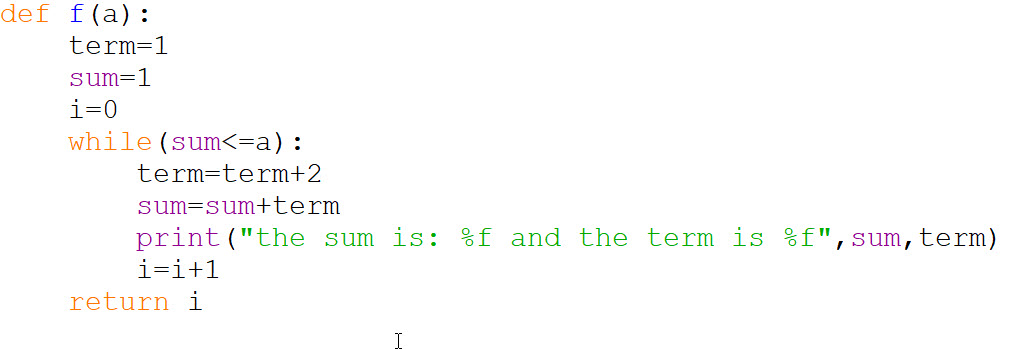
\includegraphics[width=\textwidth]{pythoncode}
\caption{
تعریف تابع در پایتون
}\label{pythoncode}
\end{figure}

با توجه به تعریف تابع 
$f(4)=2$
، اما اگر 
$a=10$
و یا
 $a=-10$
 باشد، آنگا تابع چه مقداری را برمی گرداند.
 \\
 برای درک بهتر کد پایتون شکل \ref{pythoncode} می توان نام تابع را به
  $ iroot $
تغییر داد و یک خط توضیحات به آن اضافه کرد (شکل \ref{pythoncodewithcomment}).

\begin{figure}[!t]
\centering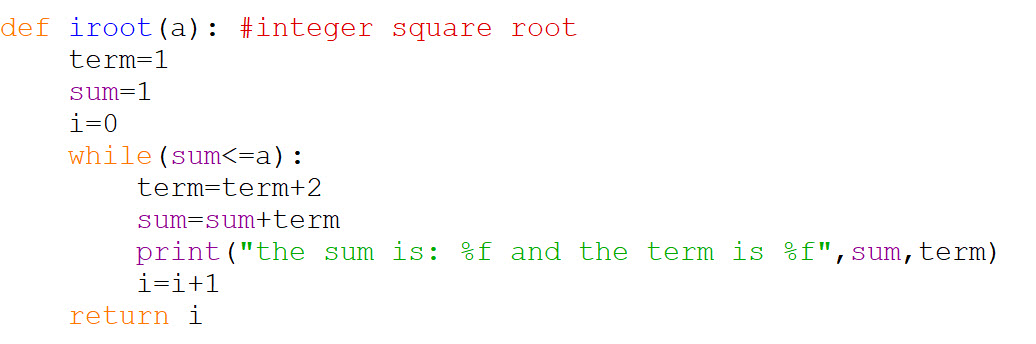
\includegraphics[width=\textwidth]{pythoncodewithcomment}
\caption{
تعریف تابع در پایتون به همراه توضیحات بیشتر
}\label{pythoncodewithcomment}
\end{figure}


 در اینجا متوجه می شویم که در توضیح این تابع، به چیزی بیشتر از کد نیاز داریم. کد، نحوه محاسبه خروجی را نشان می دهد در حالیکه "توصیف" نتیجه محاسبه را دربردارد. توصیف کد شکل
 \ref{pythoncode}
به زبان توصیف رسمی Z، به شکل \ref{iroot} خواهد بود.

\begin{figure}
\centering
\begin{schema}{iroot}
iroot :   \mathbb{N} \longrightarrow \mathbb{N}
\where
\forall a: \mathbb{N}\\
iroot(a) \ast iroot(a) \leq a < ( iroot ( a ) +1 ) \ast ( iroot ( a ) +1 )\\
\end{schema}
\caption{توصیف کد پایتون بوسیله زبان توصیف رسمی Z}
\label{iroot}
\end{figure} 
از توصیف رسمی، نمی توان به کد رسید. در توصیف برنامه، مشخص می شود که برنامه چه کاری انجام خواهد داد و در واقع به پرسش 
$ what $
پاسخ داده خواهد شد. اما کد پایتون برنامه مشخص می کند که چگونه این کار انجام می شود و پاسخ به پرسش
$ How $
را دربردارد. این دو تکمیل کننده یکدیگرند و در طراحی یک سیستم و یا یک نرم افزار، به هر دو نیاز داریم.
از مثال مطرح شده می توان به این نتیجه رسید که زبان های توصیف رسمی، زبان برنامه نویسی نیستند به این معنا که برای آنها کامپایلری که بتواند کد قابل اجرا تولید کند، وجود ندارد.

\chapter{معرفی Z}\label{chapter2}
\paragraphfootnotes
Z یک زبان توصیف رسمی مدل گراست که در دهه 80 توسط گروه پژوهشی برنامه نویسی دانشگاه آکسفورد، توسعه داده شد.این زبان مبتنی بر تئوری مجموعه Zermelo است. Z در سال 2002، استاندارد ISO را دریافت کرد.از آن زمان تاکنون، Z در طیف گسترده ای از نرم افزارهای سیستمی مانند سیستم های پایگاه داده، سیستم های تراکنشی، سیستم های محاسبات توزیع شده و سیستم عامل ها بکار برده شده است. موفقیت قابل توجه Z در توصیف فاصل برنامه نویسی کاربردی CICS بود که بوسیله آزمایشگاه IBM در پارک Hursley انجام شد. تقریبا 3700 خط کد توسط Z تولید شد. این پروژه یک پروژه صنعتی بود که توصیف آن توسط Z منجر به کاهش 5.2 درصدی خطا نسبت به حالتی که توصیف Z وجود نداشته باشد، گردید. توصیف های Z ریاضیاتی هستند و از منطق دومقداری استفاده می کنند. استفاده از ریاضیات، صحت این زبان را تضمین می کند و به شناسایی تناقضات موجود در توصیف ها، کمک می کند.
Z یک رویکرد مدل گرا است که یک مدل صریح از حالت ماشین انتزاعی را نشان می دهد. عملگرها در این حالت تعریف شده اند. ریاضیات، در Z برای نشان گذاری توصیف های رسمی و حساب شِما، برای ساختار این توصیف ها بکار می روند. شِماها از نظر بصری قابل توجه هستند و بخش اصلی آنها شامل جعبه هایی است. شِماها برای توصیف حالات و عملیات بکار می روند. حساب شِما، به شِماها این قابلیت را می دهد که با دیگر شِماها ترکیب شوند و یا در کنار هم بلوک ها را بسازند.تصویر 1، یک شِمای ساده را توصیف می کند. این شِما، توصیف ریشه مرتبه دوم مثبت یک عدد حقیقی است. 

عملگرهای شِما بصورت پیش شرط/پس شرط تعریف می شوند. یک پیش شرط باید قبل از اینکه عملگر اجرا شود، بررسی شود در حالیکه پس شرط، پس از اجزای عملگر بررسی می شود. مسلما پس از اثبات درستی پیش شرط ها، عملگر اجرا خواهد شد.پیش شرط بصورت ضمنی در داخل عملگر تعریف شده است. هر عملگر یک فرض اثبات شده به همراه دارد که تضمین می کند درصورت درست بودن پیش شرط، عملگر، تغییرناپذیری سیستم را حفظ کند. تغییرناپذیری یکی از ویژگی های سیستم است که همواره و در هر زمانی باید درست باشد. حالت اولیه سیستم نیز بنحوی است که تغیرناپذیری سیستم برآورده شود.
\begin{figure}
\centering
\begin{schema}{SqRoot}
num? , root!: \mathbb{R}
\where
num? \geq 0\\
root! \expon 2 = num?\\
root! \geq 0
\end{schema}
\caption{توصیف تابع جذر}
\label{SqRoor}
\end{figure}
در شکل \ref{SqRoor}، پیش شرط توصیف تابع جذر بصورت 
$num? \ge 0$
است. بنابراین تابع $SqRoot$ تنها ریشه اعداد حقیقی مثبت را بدست می آورد. پس شرط های تابع جذر 
 $root!^2 = num?$ و $ root! \ge 0$ 
  هستند. این دو شرط بیان می کنند که اولا ریشه عددی مثبت است و ثانیا توان دو ریشه برابر با عدد ورودی است.
  
Z یک زبان مبتنی بر نوع است ، به این معنا که وقتی متغیری معرفی می شود، باید نوع آن نیز مشخص گردد. یک نوع، مجموعه ای از اشیا است. چندین نوع استاندارد در Z وجود دارند. این انواع عبارتند از اعداد طبیعی $\mathbb{N}$، اعداد صحیح $\mathbb{Z}$، و اعداد حقیقی $\mathbb{R}$. اعلان یک متغیر به نام x که از نوع X است، بصورت x:X انجام می گیرد.همچنین در Z امکان تعریف نوع توسط برنامه نویس نیز وجود دارد.

در توصیف های Z از قراردادهای مختلفی استفاده می شود، برای مثال $v?$ بیان کننده این است که v یک متغیر ورودی است و $v!$ بیانگر این است که v، یک متغیر خروجی است. در تابع $SqRoot$ که در بالا تعریف شد، $num?$ یک متغیر ورودی، و $root!$ یک متغیر خروجی را اعلان می کند. علامت $\Xi$ در یک شِما، نشاندهنده این است که عملگر، حالت را تغییر نمی دهد، درحالیکه علامت $\Delta$ بیانگر این است که عملگر، باعث تغییر حالت می گردد.

بسیاری از انواع داده های مورد استفاده در Z، مشابهی در زبان های برنامه نویسی استاندارد ندارند. بنابراین لازم است که ساختمان داده های توافقی، شناسایی و توصیف شوند تا درنهایت برای نمایش ساختارهای ریاضیاتی انتزاعی بکار روند. باتوجه به اینکه ساختارهای توافقی ممکن است با انتزاع تفاوت داشته باشند، عملگرهای مربوط به ساختار داده های انتزاعی، نیازمند پالایش به عملگرهای  داده های توافقی هستند. این پالایش باعث می شود که نتایج حاصل، یکسان گردد. برای سیستم های ساده، پالایش مستقیم امکان پذیر است. برای بیشتر سیستم های پیچیده، پالایش با تاخیر، بکار برده می شود که در آن یک دنباله از توصیف های توافقی افزاینده، برای توصیف های قابل اجرا، تولید می شوند.
\begin{figure}
\centering
\begin{schema}{Library}
on\_shelf, missing, borrowed : \mathbb{P} Bkd\_Id
\where
on\_shelf \cap missing = \oslash\\
on\_shelf \cap borrowed = \oslash \\
borrowed \cap missing = \oslash
\end{schema}
\caption{توصیف یک سیستم کتابخانه}
\label{Library}
\end{figure}

\begin{figure}
\centering
\begin{schema}{Borrow}
\bigtriangleup Library\\
b?:Bkd\_Id
\where
b? \in on\_shelf = on\_shelf \hide \{b?\}\\
borrowed' = borrowed \cup \{b?\}
\end{schema}
\caption{توصیف عملگر امانت گرفتن کتاب}
\label{Borrow}
\end{figure}
تصویر \ref{Borrow} نشاندهنده توصیف Z برای امانت گرفتن کتاب از یک سیستم کتابخانه است. کتابخانه شامل کتاب هایی است که در قفسه قرار دارند، کتاب هایی که به امانت رفته اند و کتاب هایی که گم شده اند. توصیف، با استفاده از مجموعه هایی که نشان دهنده کتاب های موجود در قفسه، به امانت رفته و گمشده است، کتابخانه را مدلسازی می کند. بنابراین سه زیرمجموعه مجزا از مجموعه کتاب ها وجود دارد. $Bkd-Id$ شناسه هر کدام را مشخص می کند.
\\
وضعیت سیستم با استفاده از شِمای $Library$ در شکل \ref{Library} مشخص شده است. دو عمل $Borrow$ و $Return$ می توانند بر روی حالت سیستم تاثیر بگذارند. عملگر$ Borrow$ در شکل 2-1 توصیف شده است.
نشانگذاری $\mathbb{P} Bkd-Id$ مجموعه توانی $Bkd-Id$ (مجموعه تمام زیرمجموعه های$ Bkd-Id$) را نشان می دهد. شرط مجزا بودن سه زیرمجموعه on-shelf، missing و borrowed در شِمای $Library$ تعریف شده است. این شرط با تهی بودن اشتراک دو به دوی این مجموعه ها مشخص شده است. 
پیش شرط عمل $Borrow$ (امانت دادن) این است که کتاب در قفسه موجود باشد. پس شرط آن این است که کتاب به مجموعه کتاب های به امانت رفته اضافه شود و از مجموعه کتاب های موجود در قفسه، حذف شود.  









\chapter{عناصر Z}\label{chapter3}
\paragraphfootnotes
\section{مجموعه ها}\index{sets}
یک مجموعه، دسته ای از اشیا خوش تعریف است. مجموعه ها گاهی با لیستی از تمامی عناصرشان نشان داده می شوند. به عنوان مثال مجموعه اعداد طبیعی زوج کوچتر یا مساوی 10، برابر است با
 \[
 \{2, 4, 6, 8, 10\}
 \]
مجموعه ها ممکن است با بکارگیری برخی از عملیات بر روی دیگر مجموعه ها ایجاد شوند. برای مثال مجموعه اعداد طبیعی زوج کوچکتر مساوی 10، با استفاده از عملگرهای مجموعه، بصورت زیر تعربف می شود:
\[
\{n:\mathbb{N}|n\ne0 \land n<10 \land  n  mod  2=0 \bullet n\}
\]
تعریف مجموعه فوق شامل سه بخش است. بخش اول، امضای مجموعه است که بصورت $n:\mathbb{N}$
 نشان داده شده است. بخش اول با استفاده از خط عمودی | از بخش دوم جدا می شود. بخش دوم با استفاده از یک شرط بیان بیان می شود. در مثال فوق این شرط عبارت است از 
 $n\ne o \land n<10 \land n mod 2=0 $.
 بخش دوم با استفاده از 
 $\bullet $
  از بخش سوم جدا شده است. بخش سوم یک عبارت است که در مثال فوق این عبارت $n$ می باشد. این عبارت ممکن است عبارت پیچیده تری باشد مانند 
 $\log (n^2)$ .
 
 در ریاضیات تنها یک مجموعه تهی وجود دارد. در Z یک مجموعه تهی برای هر نوع از مجموعه ها وجود دارد. ازاینرو به تعداد نامتناهی مجموعه تهی در Z وجود دارد. مجموعه تهی بصورت 
 $\varnothing [X]$
  تعریف می شود که در آن X نوع مجموعه تهی را نشان می دهد. اگر نوع واضح باشد، نیازی به نوشتن X نیست.
 
 در Z عملگرهای متنوعی برای مجموعه ها وجود دارد مانند اجتماع، اشتراک، تفاوت مجموعه ها و تفاوت متقارن. مجموعه توانی یک مجموعه مانند X، شامل تمام زیرمجموعه های مجموعه X است و با 
 $\mathbb{P}X$
 نشان داده می شود. مجموعه زیرمجموعه های غیرتهی X با 
 $\mathbb{P}_1 X$
 نشان داده می شود که در آن
 \[
 \mathbb{P}_1 ==\{ U: \mathbb{P} X|U\neq \varnothing[X]\}
 \]
 یک مجموعه متناهی از عناصر نوع X که با 
 $\bold F X$
 نشان داده می شود، زیرمجموعه ای از X است که نمی تواند یک تناظر یک به یک با زیرمجموعه خاصی از خودش داشته باشد. تعریف 
 $\bold F X$
 بصورت زیر است.
 \[
 \bold F X== \{ U:\mathbb{P}X| \neg \exists V : \mathbb{P} U \bullet V \neq U \land ( \exists f:V \to U)\}
\] 

عبارت
 $f:V\longmapsto U $
 بیان می دارد که f یک رابطه یک به یک از U به V است که در آن هر عضو از مجموعه U دقیقا به یک عضو از مجموعه V نگاشت می شود و برعکس.
 
 Z یک زبان نوع دار است به این معنا که متغیر در هنگام تعریفش، برای اولین بار اعلان می شود. تعریف متغیر با استفاده از سورهای عمومی و وجودی انجام می گردد. برای مثال 
 \[
 \forall j:J \bullet P \Rightarrow Q
 \]
 .
 
 کمیت وجودی یکتا بصورت 
 $\exists _1 j:J|P$
 تعریف می شود. این تعریف بیان می کند که دقیقا یک j از نوع J وجود دارد که دارای ویژگی P است.   



\section{رابطه ها}\index{رابطه ها}
رابطه R میان X و Y زیرمجموعه ای از ضرب کارتزین X و Y است; یعنی 
$R \subseteq (X \times Y)$.
رابطه در Z بصورت
$R: X \longleftrightarrow Y$
نمایش داده می شود. رابطه  
$ x \mapsto y$
نشاندهنده این است که زوج 
$ (x,y) \in R$.
\\
توجه کنید که رابطه 
$ home\_owner : Person \longleftrightarrow Home $
بین افراد و خانه هایشان برقرار است. رابطه 
$ daphne \longmapsto mandalay \in home\_owner $
بیان می دارد که $daphne$ مالک $mandalay$ است. همچنین امکان دارد که یک شخص بیش از یک خانه داشته باشد:
\[
rebecca \longmapsto nirvana \in home\_owner
\\
rebecca \longmapsto tivoli \in home\_owner
\]
همچنین ممکن است دو نفر بصورت مشترک مالک خانه ای باشند:
\[
rebecca \longmapsto nirvana \in home\_owner
\\
lawrence \longmapsto nirvana \in home\_owner
\] 
ممکن است افرادی وجود داشته باشند که مالک هیچ خانه ای نیستند. بنابراین، برای آنها، ورودی در رابطه $home\_owner$ وجود ندارد. نوع $Person$ شامل هر فرد ممکنی است و نوع $Home$ دربرگیرنده هر خانه ممکنی می باشد. دامنه رابطه $home\_owner$ بصورت زیر تعریف می شود:

\[
x \in  \dom \enspace  home\_owner \Leftrightarrow \exists h : Home . x \longmapsto h \in home\_owner
\]


برد رابطه $home\_owner$ را نیز می توان بصورت زیر تعریف کرد:
\[
h \in  \ran \enspace home\_owner \Leftrightarrow \exists x : Person . x \longmapsto h \in home\_owner
\]
ترکیب دو رابطه 
$home\_owner:Person\leftrightarrow Home$
و
$home\_value: Home \leftrightarrow Value$
منجر به رابطه
$owner\_wealth: Person \leftrightarrow value$
می شود. این رابطه با ترکیب رابطه ای\footnote{relational composition} 
$home\_owner ;home\_value$
نشان داده می شود که در آن
\[
p\mapsto v \in home\_owner ; home\_value  \Leftrightarrow 
\\ (\exists h: Home . p\mapsto h \in home\_owner \wedge h\mapsto v \in home\_value)
\]
ترکیب رابطه ای همچنین ممکن است بصورت زیر نشان داده شود:
\[ owner\_wealth=home\_value \circ home\_owner \]
اجتماع دو رابطه نیز گاهی در عمل مورد نیاز است. فرض کنید که یک ورودی جدید بصورت 
$aisling \mapsto muckross$
اضافه شود. این وضعیت بصورت زیر نشان داده می شود.
\[ home\_owner'= home\_owner \cup {aisling \mapsto muckross}\]
حال فرض کنید می خواهیم اسامی تمام خانم هایی را که مالک خانه هستند، داشته باشیم. بنابراین باید رابطه
$home\_owner$
را محدود به حالاتی کنیم که عنصر اول زوج مرتب های آن، خانم باشند. توجه کنید که داریم
$female: \pset Person$
و
$\{aisling , rebecca\} \subseteq female$
.
\[home\_owner =\{aisling \mapsto muckross, rebecca \mapsto nirvana,
\\ lawrence \mapsto nirvana\}\]
\[female \triangleleft home\_owner =\{ aisling \mapsto muckross , rebecca \mapsto nirvana\}\]
$female \triangleleft home\_owner$
رابطه ای است که زیر مجموعه $home\_owner$ است و در این رابطه ، اولین عنصر هر زوج مرتبی، $female$ است. عملگر  
$\triangleleft$
محدود کننده دامنه عبارت \footnote{termed domain restriction}
است و ویژگی اصلی آن بصورت زیر بیان می شود:
\[ x\mapsto y \in U \triangleleft R \Leftrightarrow (x \notin U \wedge x\mapsto y \in R)\]
که در آن
$R: X \leftrightarrow Y$
و
$U : \pset X$
.
عملگر دیگری تحت عنوان عملگر ضدمحدودیت دامنه \footnote{domain anti-restriction}
وجود دارد که ویژگی اصلی آن بصورت زیر توصیف می شود:
\[ x\mapsto y \in U \ndres R \Leftrightarrow (x \notin U \wedge x\mapsto y \in R)\]
که در آن
$R: X \leftrightarrow Y$
و
$U : \pset X$
. 
همچنین عملگرهای محدودیت برد \footnote{range restriction}
با نماد $\triangleright$ و  ضدمحدودیت برد \footnote{range anti-restriction}
با نماد $\rsub$ در زبان Z مورد استفاده قرار می گیرند. این عملگرها تعاریفی مشابه عملگرهای دامنه دارند با این تفاوت که برای برد تابع $x\mapsto y$ محدودیت ایجاد می کند.


\section{توابع}
یک تابع، بیانگر وابستگی بین اشیا نوع X با اشیا نوع Y می باشد که در آن هر شی از نوع X، تنها به یک شی از نوع Y وابسته است. به بیان دیگر می توان گفت که یک تابع مجموعه ای از زوج مرتب هاست که در آنها عنصر اول هر زوج مرتب، حداکثر با یک عنصر رابطه دارد. درحقیقت تابع نوع خاصی از رابطه است که در آن هریک از عناصر مجموعه دامنهف تنها با یک عنصر از مجموعه برد، می توانند رابطه داشته باشند. تابع ممکن است کامل یا جزئی باشد.
\\
یک تابع جزئی از X به Y که به صورت
$ f: X\nrightarrow Y$
نشان داده می شود، تابع 
$f: X' \longrightarrow Y$
برای یک زیرمجموعه سره $X'$ از X است. اگر زیرمجموعه $X'$ سره نباشد، یعنی اگر $X'=X$ 
، تابع f را یک تابع کامل می گوییم. از توابع جزئی معمولا زمانی استفاده می شود که دامنه یک تابع مشخص نیست.
تابع جزئی بصورت زیر تعریف می شود:
\[
\forall x:X ; y,z: Y . (x\longmapsto y \in f\wedge x \longmapsto z \in f \Rightarrow y=z)
\]
وابستگی بین x و y بصورت  $f(x)=y$ نشان داده می شود. این بدان مفهوم است که مقدار تابع جزئی f برای x، برابر y است. تابع کامل از X به Y، که با $f: X\rightarrow Y$ نشان داده می شود، یک تابع جزئی است که در آن هر عنصر مجموعه X به یک مقدار از مجموعه Y وابسته شده است.
\[
f: X \rightarrow Y \Leftrightarrow f: X\nrightarrow Y \wedge \dom f=X
\]
واضح است که هر تابع کامل، یک تابع جزئی است ولی هر تابع جزئی، یک تابع کامل نیست.
\begin{figure}
\centering
\begin{schema}{TempMap}
CityList : \pset City
\\
temp: City \nrightarrow Z
\ST
\dom temp = CityList
\end{schema}
\label{TempMap}
\end{figure}
عملگری که از تکرار در توصیف ها ناشی می شود، عبارت است از عملگر لغو
\LTRfootnote{override}
. به توصیف نگاشت دمایی که در 
\ref{TempMap}
 آمده است توجه کنید.یک مثال از نگاشت دما بصورت زیر می تواند باشد:
\[
 temp= \{ Cork \mapsto 17, Dublin \mapsto 19, London \mapsto 15\}
\]
حال مساله بروزرسانی دما مطرح می گردد، زمانیکه مثلا می خواهیم دمای Cork را تغییر دهیم. برای مثال
$(Cork \mapsto 18)$
.
بنابراین یک نمودار دمای جدید با استفاده از نمودارهای قدیمی و عملگر لغو تابع خواهیم داشت که نتیجه آن 
\[
\{ Cork \mapsto 18, Dublin \mapsto 19, London \mapsto 15\}
\]
است. این عملیات بصورت زیر نوشته می شود:
\[
temp' = temp \oplus {Cork \mapsto 18}
\]
عملگر لغو تابع، دو تابعی را که از دارای یک نوع هستند باهم ترکیب کرده و تابع جدیدی با همان نوع ایجاد می کند. تاثیر عملگر لغو به این صورت است که ورودی
$\{ Cork \rightarrow 17\}$
از نمودار دما را حذف می کند و با ورودی 
$\{ Cork \rightarrow 18 \}$
جایگزین می کند.
\\
فرض کنید 
$ f,g: X \nrightarrow Y$
دو تابع جزئی هستند. 
$f\oplus g$
اینگونه تعریف می شود که f بوسیله g لغو شده است. تعریف 
$f\oplus g$
بصورت زیر است: 
\[
(f \oplus g)(x) = g(x) where x \in \dom g
\\
(f \oplus g)(x)= f(x) where x \notin \dom g \wedge x \in \dom f
\] 
این عملگر همچنین ممکن است بصورت زیر تعریف شود:
\[
 f\oplus g =((\dom g) \ndres f) \cup g
 \]
 در Z امضاهایی برای توابع injective، bijective و surjective وجود دارد. تابع injective یک تابع یک به یک است.
 \[
 f(x)=f(y) \Rightarrow x=y
 \]
 تابع surjective بصورت زیر تعریف می شود:
 \[
 Given  y \in Y , \exists  x \in X such  that f(x)=y
 \]
 تابع bijective نیز یک تابع یک به یک است که نشان می دهد مجموعه های X و Y با یکدیگر تناظر یک به یک دارند.
  \\
  Z شامل نشانگذاری عبارت لامبدا\footnote{Lambda}، برای تعریف توابع است.
  برای مثال تابع:
  \[ 
  cube== \lambda x:N \bullet x*x*x
  \]
  ترکیب توابع f و g مشابه ترکیب روابط است.
  
  
\section{دنباله ها}
نوه تمامی دنباله های عناصر از یک مجموعه مانند $X$ف با نماد $seq X$ نشان داده می شود. دنباله بصورت 
$< x_1,x_2, ..., x_n>$
نمایش داده می شود. دنباله تهی به صورت $<>$ نشان داده می شود. دنباله ها ممکن است برای نشان دادن تغیر حالت یک متغیر در طول زمان، بکار برده شوند که در آن هر عنصر دنباله، نشاندهنده مقداری از متغیر در زمان های گسسته است.
\\
 دنباله ها همان توابع هستند  و یک دنباله از عناصر روی مجموعه $X$ ، یک تابع متناهی  از مجموعه اعداد طبیعی به $X$ است. یک تابع جزئی متناهی به نام $f$ از $X$ به $Y$ بصورت
 $f: X \ffun Y$
 تعریف می شود.
 \\
 یک دنباله متناهی از عناصر $X$ بصورت 
 $f: N \ffun X$
 نشان داده می شود. دامنه این تابع شامل تمام اعداد بین 1 و 
 $\#f$
  است که در آن 
 $\# f$
 کاردینالیتی $f$ است. این موضوع با استفاده از فرمول زیر نشان داده می شود.
 \[seq \enspace X==\{f:N \ffun X | \dom \enspace f=1 .. \#f \bullet f\}\]
 دنباله 
 $<x_1,x_2, ...,x_n>$
  که در بالا معرفی شد بصورت
$\{1\longmapsto x_1, 2\longmapsto x_2, ... , n\longmapsto x_n \}$  
  تعریف می شود.
  \\
  عملگرهای متنوعی برای دستکاری کردن دنباله ها وجود دارند. یکی از این عملگرها، عملگر الحاق است. فرض کنید 
  $\sigma = < x_1, x_2, ... , x_n>$
  و
  $\tau =<y_1, y_2, ..., y_n>$
  دو دنباله مفروض باشند. آنگاه
  \[\sigma \cap \tau = <x_1, x_2, ..., x_n, y_1, y_2, ..., y_n>\]
  سرآیند \footnote{hesd} یک دنباله غیرتهی، اولین عنصر آن دنباله است.
 \[heads \enspace \sigma =head <x_1, x_2, ..., x_n> = x_1\]
 ته\footnote{tail} یک دنباله غیرتهی، شامل تمامی عناصر دنبالهف غیر از عنصر اول آن، می باشد.
 \[tail \enspace \sigma = tail <x_1, x_2, ..., x_n> = <x_2, x_3, ..., x_n>\]
 فرض کنید
 $f: X \longrightarrow Y$
 و یک دنباله بصورت
 $\sigma : seq X$
 وجود دارد. آنگاه تابع نگاشت \footnote{map} $f$ را برای تمام عناصر $\sigma$ بکار می برد:
 \[ map \enspace f \enspace \sigma = map f <x_1, x_2, ..., x_n> = <f(x_1), f(x_2), ... f(x_n)>\]
 تابع نگاشت، همچنین با استفاده از ترکیب توابع بصورت زیر تعریف می شود:
 \[ map \enspace f \enspace \sigma = \sigma ; f\]
 معکوس\footnote{reverse} یک دنباله با استفاده از تابع $rev$ بدست می آید:
 \[rev \enspace \sigma = rev <x_1, x_2, ..., x_n> = <x_n, ..., x_2, x_1> \]
 
 \section{کیسه ها}
 کیسه\footnote{bag} مشابه مجموعه است با این تفاوت که کیسه می تواند عنصر تکراری داشته باشد. یک کیسه از عناصر نوع X بصورت یک تابع جزئی تعریف می شود که دامنه آن، از نوع عناصر موجود در کیسه و برد آن، تمام اعداد مثبت است. تعریف یک کیسه از نوع $X$ بصورت زیر است:
 \[bag \enspace X= X \nrightarrow \mathbb{N}_1.\]
 به عنوان مثال یک کیسه از مهره ها را در نظر بگیرید. این کیسه ممکن است شامل 3 مهره آبی، 2 مهره قرمز و یک مهره سبز باشد. این کیسه را می توان بصورت 
$B=[b, b, b, g, r, r]$ 
 نشان داد. این کیسه از مهره ها همچنین بصورت زیر تعریف می شود:
 \[ bag \enspace Marbel == Marbel \nrightarrow \mathbb{N}_1.\]
 تابع $count$ تعداد رخدادهای یک عنصر موجود در کیسه را مشخص می کند. به عنوان مثال، در کیسه فوق،
 $count \enspace Marbel \enspace b=3$
 و
$count \enspace Marbel \enspace y=0$ 
،بنابراین هیچ مهره زردی در کیسه وجود ندارد. این مطلب  با استفاده از فرمول های زیر بیان می شود:
\[count \enspace bag X \enspace y=0 \hspace{80pt} y\notin bag \enspace X\\
count \enspace bag X \enspace y=(bag X)(y) \hspace{35pt} y\in bag \enspace X\]
عضو $y$ در کیسه $X$ قرار دارد اگر و فقط اگر $y$ در دامنه کیسه $X$ باشد:
\[y \enspace in \enspace bag X \Leftrightarrow y \in \dom(bagX)\]
اجتماع دو کیسه 
$B_1=[b, b, b, g, r, r]$
و
$B_2=[b, g, r, y]$
بصورت
$B_1\uplus B_2=[b, b, b, b, g, g, r, r, r, y]$
نوشته می شود. عمل اجتماع با استفاده از فرمول های زیر توصیف می شود:
\[
(B_1\uplus B_2)(y)=B_2(y) \hspace{70pt} y\notin \dom \enspace B_1 \wedge y\in \dom \enspace B_2\\
(B_1\uplus B_2)(y)=B_1(y) \hspace{70pt} y\in \dom \enspace B_1 \wedge y\notin \dom \enspace B_2\\
(B_1\uplus B_2)(y)=B_1(y)+B_2(y) \hspace{30pt} y\in \dom \enspace B_1 \wedge y\in \dom \enspace B_2
\]
\begin{figure}
\centering
\begin{schema}{\bigtriangleup Borrow}
stock : bag \enspace Good\\
price: Good\rightarrow \mathbb{N}_1
\where
\dom \enspace stock \subseteq \dom \enspace price
\end{schema}
\caption{توصیف دستگاه فروش با استفاده از کیسه}
\label{Borrow}
\end{figure}
 کیسه ممکن است برای ضبط تعدا موجودی هر محصول در یک انبار که بخشی از یک سیستم فروش است، بکار برده شود. شمای فوق (شکل\ref{Borrow})، تعداد اقلام باقیمانده از هر محصول را در یک سیستم فروش، مدلسازی می کند.
 \\
 عملیات یک ماشین فروش نیازمند عملگرهایی نظیر عملگر شناسایی مجموعه سکه های قابل قبول، بررسی کافی بودن مبلغ ورودی متناسب با قیمت کالا، بازگرداندن مبلغ اضافی به مشتری، و بروزرسانی مقدار موجود از هر کالا پس از انجام عملیات خرید، می باشد.
 \section{شِما و ترکیب شِما} 
توصیف Z در یکسری جعبه های بصری ارائه می شود که آنها را شِما یا سکیما\footnote{schema} گویند. این جعبه ها در حالت های خاصی به کار می روند . نشان گذاری هایی را برای نمایش حالت قبل و حالت بعد، بکار می گیرند. (به عنوان مثال s و s' که در آن s' حالت بعد از s است). شِماها، تمامی اطلاعات مرتبط باهم را برای شرح یک حالت، گروهبندی می کنند.
\\
عمگرهای مفیدی برای کار با شِماها وجود دارند مانند عملگر شمول شما\footnote{$schema \enspace inclusion$}، عملگر ترکیب شِما \footnote{schema composition} و استفاده از اتصال گزاره ها برای متصل کردن شِماها به یکدیگر.
\\
نماد $\Delta$ بصورت قراردادی نشاندهنده این است که شِمای حاضر بر حالت تاثیر می گذارد. در مقابل عملگر $\Xi$ به این معناست که حالت از شِما تاثیر نمی پذیرد. این قراردادها، قابلیت خوانایی توصیف را افزایش می دهند و امکان تعریف عملگرهای پیچیده تر را فراهم می کنند.
\\
عملگر ترکیب شِما باعث می شود که شِماهی جدیدی از شِماهای موجود مشتق گردد. شِمایی با نام $S_1$ ممکن است در بخش اعلان شِمای $S_2$ مورد استفاده قرار گیرد. تاثیر شمول به این نحو است که اعلان های موجود در $S_1$ ، حالا بخشی از اعلان های $S_2$ هستند و گزاره های $S_1$ و $S_2$ با یکدیگر ترکیب عطفی شده اند. اگر یک متغییر هم در $S_1$ و هم در $S_2$ تعریف شده باشد، باید نوع آن در هر دو شما یکسان باشد. 




\begin{schema}{S_1}
x,y: \enspace \mathbb{N}
\where
x+y > 2
\end{schema}

\begin{schema}{S_2}
S_1 ; z: \mathbb{N}
\where 
z=x+y
\end{schema}
نتیجه اینکه
 $S_2$
  شامل اعلان ها و گزاره های
   $S_1$
   است (تصویر \ref{fig 3-2}).

\begin{figure}
\centering
\begin{schema}{S_2}
x,y : \enspace \mathbb{N}
\\
z:\mathbb{N}
\where
x+y >2
\\
z=x+y
\end{schema}
\caption{شمول دو شِما}
\label{fig 3-2}
\end{figure}
دو شِما ممکن است توسط اتصال های گزاره ای نظیر 
$S_1 \land S_2$
،
$S_1 \wedge S_2$
،
$S_1 \Rightarrow S_2$
و یا
$S_1 \Leftrightarrow S_2$
به یکدیگر متصل شوند.
شِمای 
$S_1 \wedge S_2$
 باعث می شود که بخش اعلان دو شِمای $S_1$ و $S_2$ با یکدیگر ادغام شوند و سپس گزاره های آنها نیز بوسیله عملگر منطقی ترکیب فصلی $\wedge$ با یکدیگرف ترکیب شوند. برای مثال 
 $S=S_1 \wedge S_2$
 در شکل \ref{fig 3-3} نشان داده شده است.
 

 
\begin{figure}
\centering
\begin{schema}{S}
x,y : \enspace \mathbb{N}
\\
z:\mathbb{N}
\where
x+y >2 \wedge z=x+y
\end{schema}
\caption{ترکیب فصلی دو شمای $S_1$ و $S_2$}
\label{fig 3-3}
\end{figure}

دو عملگر شمول شِما و اتصال شِماها، برای تبدیل زیر نوع ها به انواع بیشینه، از نرمال سازی استفاده می کنند. از طرفی گزاره ها نیز برای محدود کردن انواع بیشینه به زیرنوع ها بکار می روند. این عمل منجر به جایگزینی اعلان متغیرها می شود. به عنوان مثال 
$u: 1 . . 35$ با $u:\mathbb{Z}$ جایگزین می شود و گزاره 
$u>0 \enspace and \enspace u<36$
به بخش گزاره شِما اضافه می گردد.
\\
دو نماد $\Delta$ و $\Xi$ به کرات در تعریف شِماها بکار می روند. وقتی که نشان گذاری 
$\Delta TempMap$
 در توصیف یک شِما، دیده می شود به این مفهوم است که این شِما، حالت را تغییر می دهد.
 \[ 
 \Delta TempMap= TempMap \land TempMap'
 \]
 شکل مفصل تر $\Delta TempMap$  در تصویر\ref{fig 3-4} توصیف شده است.
 
 \begin{figure}
\centering
\begin{schema}{\Delta TempMap}
CityList, CityList' : \enspace \mathbb{P}\enspace City
\\
temp , temp': \enspace City\nrightarrow Z
\where
\dom temp =CityList
\\
\dom temp'=CityList'
\end{schema}
\caption{کاربرد عملگر $\Delta$}
\label{fig 3-4}
\end{figure}

نشان گذاری $\Xi$ برای توصیف عملگرهایی استفاده می شود که منجر به تغییر حالت نمی شوند. نمونه ای از این نشان گذاری در شکل \ref{fig 3-5} قابل مشاهده است.

\begin{figure}
\centering
\begin{schema}{\Xi TempMap}
\Delta TempMap
\where
CityList =CityList'
\\
temp=temp'
\end{schema}
\caption{کاربرد عملگر $\Xi$}
\label{fig 3-5}
\end{figure}

عملگر ترکیب شِما باعث می شود که توصیف های جدیدی از روی توصیف های موجود ساخته شوند. ترکیب شِما، مقادیر حالت بعدی یک شِما را به مقادیر حالت قبلی شِمای دیگری، ربط می دهد. ترکیب دو شِمای $S$ و $T$ 
،
$(S;T)$
شامل چهار مرحله است که در جدول
\ref{tab3-1}


نشان داده شده است.
\begin{table}[!t]
\centering
\caption{
مراحل ترکیب شِما
}
\begin{tabular}{cc}
\toprule
گام & روال  
\\
\midrule
1. &  تمامی مقادیر حالت "بعدی" موجود در $S$، با نام های جدید، بازنامگذاری می شوند:
 $S[s^+ / s']$
\\
2. & تمامی مقادیر حالت "قبلی" موجود در $T$ با همان نام های جدید، بازنامگذاری می شوند:
$S[s^+ / s]$
\\
3. & ترکیب عطفی دو شِمای جدید ایجاد می شود:
$S[s^+/s'] \land T[s^+/s] $
\\
4.& متغیرهایی که در گام های 1 و 2 معرفی شده اند، مخفی می شوند.
$ S;T=(S[s^+/s'] \land T[s^+/s]) (s^+) $

\\ \bottomrule
\end{tabular}
\label{tab3-1}
\end{table}


چهار شمای $S$، $T$، $T_1$ و $S_1$  در شکل 
\ref{fig 3-6}
نشان داده شده است.
\begin{figure}
\centering
\begin{schema}{S}
x,x',y ? : \mathbb{N}
\where
x'=y?-2
\end{schema}

\begin{schema}{T}
x,x'  : \mathbb{N}
\where
x'=x+1
\end{schema}

\begin{schema}{S_1}
x,x^+, y?  : \mathbb{N}
\where
x^+=y?-2
\end{schema}

\begin{schema}{T_1}
x^+, x': \mathbb{N}
\where
x'=x^+1
\end{schema}
\caption{معرفی چهار شِمای $S$، $T$، $S_1$ و $T_1$}
\label{fig 3-6}
\end{figure} 

 این شِماها در تصویر
\ref{fig 3-7}
با یکدیگر ترکیب شده اند.




$S_1$ و $T_1$ نتایج گام های 1 و 2 را نشان می دهند. 
$x'$ در $S$ با $s^+$ بازنامگذاری شده است و $x$ در $T$ با $x^+$ بازنامگذاری شده است. نتایج گام های 3 و 4 را نیز در تصویر
\ref{fig 3-7}
می توانید مشاهده کنید.

\begin{figure}[ht]
\centering

\begin{schema}{S_1 \land T_1}
x,x^+, x', y? : \mathbb{N}
\where
x^+=y?-2\\
x'=x^+1
\end{schema}



\begin{schema}{S;T}
x, x', y? : \mathbb{N}
\where
\exists x^+: \mathbb{N} \bullet \\
(x^+=y?-2
\\x' = x^+ +1)
\end{schema}

\caption{ترکیب شِما}
\label{fig 3-7}
\end{figure} 
\chapter{ چند نمونه ساده توصیف Z}\label{chapter4}


\section{نمونه اول: کتابچه تولد}\index{sample1}
بهترین راه برای درک زبان $Z$ مطالعه نمونه های ساده است. به عنوان اولین نمونه، سیستمی پیاده سازی می شود که در آن کتابچه تولد، به جای استفاده از دفترچه و خودکار، توسط یک سیستم کامپیوتری ایجاد می شود. در این سیستم، تاریخ تولد افراد ثبت می شود و سیستم قادر است که با نزدیک شدن روز تولد افراد، آن را یادآوری کند.\\
شخصی که می خواهد برای خود در سیستم کتابچه تولد، یک حساب کاربری ایجاد کند، باید نام افراد و تاریخ تولد آنها را ثبت کند.  بنابراین مجموعه ای از نام ها و مجموعه ای از تاریخ ها را، به عنوان نوع اصلی، در این توصیف خواهیم داشت.\\
 \[
 [NAME, DATE]
 \]
 \\
 تعریف این دو مجموعه باعث می شود که بتوان مجموعه ها را بدون بیان صریح نوع اشیایی که شامل می شوند، نامگذاری کرد.  \\
 اولین جنبه سیستم، تشریح فضای حالت آن است که با استفاده از شمای شکل 
 \ref{fig4-1}
 توصیف شده است.\\
\begin{figure}
\centering
\begin{schema}{\mathit{BirthdayBook}}
\mathit{known} :\mathbb{P}\enspace NAME\\
\mathit{birthday} : NAME \nrightarrow DATE
\ST
\mathit{known} = \dom \enspace \mathit{birthday}\\
\end{schema}
\caption{}
\label{fig4-1}
\end{figure}
مشابه دیگر شِماها، این شِما نیز شامل دو بخش است که با یک خط تقسیم مرکزی از یکدیگر جدا شده اند. در بخش بالا، متغیرها اعلان شده اند و در بخش پایین، رابطه بین متغیرها و مقادیرشان مشخص شده است. در این مورد، فضای حالت سیستم و دو متغیری که نشاندهنده مشاهدات بااهمیت هستند و می توانند حالت ها را ایجاد کنند، تشریح شده اند:
\\
$\bullet known:$
مجموعه ای از نام هاست که تاریخ تولد آنها ثبت شده است.
\\
$\bullet birthday:$
تابعی است که زمانیکه نام معینی مشخص می شود، تاریخ تولد منتسب به آن را می دهد.

 
بخشی از شِما که در زیر خط قرار دارد، رابطه ای را نشان می دهد که در تمامی حالت های سیستم، درست است و با پس از اعمال عملگرها نیز همچنان این رابطه درست باقی می ماند. در این مثال، رابطه بیانگر این است که مجموعه $known$ مشابه دامنه تابع $birthday$ است. این متغیر شامل مجموعه ای از نامهاست که برای آنها تاریخ تولدی ثبت شده است. این رابطه، در سیستم غیرقابل تغییر است.
\\

در این مثال، غیرقابل تغییر بودن، به مقدار متغیر $known$ اجازه می دهد که از مقدار  $birthday$ مشتق شود. در واقع $known$ یک مولفه مشتق شده از حالت است و می توان سیستم را بدون اشاره به $known$ مشخص کرد. البته باید توجه داشت که دادن نام ها، خوانایی توصیف را افزایش می دهد زیرا یک دید انتزاعی از فضای حالت کتابچه تولد را ایجاد می کند.
\\
یکی از حالت های ممکن سیستم حالتی است که شامل سه نفر در مجموعه $known$ است که تاریخ های تولد آنها با استفاده از تابع $birthday$ ثبت شده است:

\[
\mathit{known} = \{John, Mike, Susan\}
\]
\[
\mathit{birthday} = \{John\mapsto 25-Mar,\\
\hspace{60pt} Mike \mapsto 20-Dec,\\
\hspace{60pt} Susan \mapsto 20-Dec\}.\\
\]

ویژگی غیرقابل تغییر بودن در مثال فوق ارضا می شود زیرا تابع $birthday$ دقیقا برای هر سه اسم نام موجود در $known$، یک روز را ثبت کرده است.
\\
توجه کنید که در شرح فضای حالت سیستم، محدودیتی برای تعداد زمان تاریخ تولدهای ثبت شده در کتابچه تولد، قرار داده نشده است. همچنین فرمت خاصی برای ورود نام ها و روزهای تولد تعریف نشده است. از طرف دیگر برای هر فرد تنها یک تاریخ تولد ثبت می شود زیرا که $birthday$ یک تابع است، اما برای دو نفر متفاوت ممکن است یک تاریخ تولد ثبت شود (همانشور که در مثال فوق نیز این اتفاق رخ داده است).
\\
در ادامه عملگرهای سیستم تعریف خواهند شد. اولین عملگر، عملگری است که امکان اضافه کردن یک تاریخ تولد جدید را فراهم می کند. این عملگر در شِمای شکل\ref{AddBirthday} 
توصیف شده است.

\begin{figure}
\centering
\begin{schema}{\mathit{AddBirthday}}
\vartriangle \mathit{BirthdayBook}\\
\mathit{name?}:NAME \\
\mathit{date?}: DATE \\
\ST
\mathit{name?} \notin \mathit{known}\\
\mathit{birthday'}=\mathit{birthday}\cup \{\mathit{name?}\mapsto \mathit{date?}\}
\end{schema}
\caption{}
\label{AddBirthday}
\end{figure}

اعلان 
$\vartriangle \mathit{Birthday}$
بیانگر این مطلب است که این شِما، یک تغییر حالت را توصیف می کند. در این شِما چهار متغیر معرفی می شوند: 
$\mathit{known}$،
$\mathit{birthday}$،
$\mathit{known'}$ و
$\mathit{birthday'}$.
دوتای اول مربوط به مشاهدات حالت، قبل از تغییر و دوتای بعدی، مربوط به مشاهدات حالت، بعد از تغییر هستند.
هر زوج متغیر، محدودیت غیرقابل تغییر بودن را ارضا می کنند.
سپس دو ورودی عملگر، اعلان می شوند. برای اعلان ورودی ها، پس از اعلان نام ورودی، علامت سوال گذاشته می شود.
\\
بخشی از شِما که در زیر خط قرار گرفته است، ابتدا به بیان یک پیش شرط برای انجام موفقیت آمیز عملگر می پردازد، به این ترتیب که نامی که می خواهد اضافه شود نباید قبلا در سیستم ثبت شده باشد. این پیش شرط منطقی به نظر می رسد زیرا به ازای هر نفر تنها یک تاریخ تولد باید در سیستم ثبت شود. اینکه اگر پیش شرط برآورده نشود، چه اتفاقی خواهد افتاد، در این توصیف مشخص نشده است.
\\ اگر پیش شرط برآورده شود در خط بعدی تابع 
$\mathit{birthday}$
توسعه داده می شود و یک نام جدید به تاریخ تولدش نگاشت می شود.
انتظار می رود که نام جدید نیز به مجموعه نام های موجود در سیستم اضافه شود.
\[
\mathit{known'}=\mathit{known} \cup \{ \mathit{name?}\}.
\]

درواقع این مطلب از توصیف 
$\mathit{AddBirthday}$
، با استفاده از ویژگی غیرقابل تغییر بودن حالت، پیش و پس از اعمال عملگر، قابل اثبات است.
\[
\mathit{known'}= \dom \enspace \mathit{birthday'} \\
\hspace*{37pt} =\dom \enspace (\mathit{birthday} \cup \{ \mathit{name?}\mapsto \mathit{date?}\}) \\
\hspace*{37pt} =\dom \enspace \mathit{birthday} \cup \dom \{ \mathit{name?}\mapsto \mathit{date?}\}\\
\hspace*{37pt} =\dom \enspace \mathit{birthday} \cup  \{ \mathit{name?}\}\\
\hspace*{37pt} = \mathit{known} \cup  \{ \mathit{name?}\}\\
\]
ویژگی های اثبات و حالت، مانند آنچه که در بالا ذکر شد، تضمین میکنند که توصیف ها از دقت بالایی برخوردارنند که در نهایت منجر به توسعه سیستم هایی می گردد که درنهایت رفتاری بدون اشکال خواهند داشت.
\\
 دو واقعیت درخصوص 
 $dom$
 در این استدلال وجود دارد که مثالی از یک قانون ریاضی است. این قانون عبارت است از:
 \[
 dom(\mathit{f\cup g})= (dom \enspace \mathit{f}) \cup (dom \enspace \mathit{g})\\
 dom\{\mathit{a \mapsto b}\}= \{ \mathit{a}\}.
 \]
 عملگر دیگری که برای یافتن روز تولد افراد بکار می رود، با استفاده از شِما شکل \ref{FindBirthday}  تعریف شده است.
\begin{figure}
\centering
\begin{schema}{\mathit{FindBirthday}}
\Xi \mathit{BirthdayBook}\\
\mathit{name?}:NAME \\
\mathit{date!}: DATE \\
\ST
\mathit{name?} \in \mathit{known}\\
\mathit{date!}=\mathit{birthday}(\mathit{name?})
\end{schema}
\caption{}
\label{FindBirthday}
\end{figure}
در شِمای شکل \ref{FindBirthday} دو علامت جدید دیده می شود. اعلان 
$\Xi \mathit{BirthdayBook}$
بیانگر این است که این عملگر منجر به تغییر حالت نخواهد شد. به این معنا که مقدار $\mathit{known'}$
و
$\mathit{birthday'}$
، در مشاهدات بعد از اعمال عملگر، برابر است با مقدار 
$\mathit{kKnown}$
 و
$\mathit{birthday}$
 قبل از اعمال عملگر. استفاده از 
 $\Xi \mathit{BirthdayBook}$
 در خط اول شِما تاثیری مشابه این دارد که در خط اول 
 $\vartriangle \mathit{BirthdayBook}$
 آورده شود و دو تساوی زیر نیز در ادامه و در زیر آن نوشته شوند:
 \[
 \mathit{known'} = \mathit{known}\\
 \mathit{birthday'}= \mathit{birthday}
 \]
 علامت جدید دیگری که در این شِما استفاده شده است، نمادی است که بعد از $\mathit{date}$ آمده است و تعیین می کند که این متغیر یک خروجی است. عملگر 
 $\mathit{FindBirthday}$
  نام را به عنوان ورودی دریافت م کند و تاریخ تولد متناسب با آن را به عنوان خروجی، می دهد. پیش شرطی که برای انجام موفقیت آمیز این عملگر مورد نیاز است این است که 
  $\mathit{name?}$
   یکی از نام های موجود در سیستم باشد. در اینصورت خروجی 
   $\mathit{date!}$
    برابر است با مقدار تابع $\mathit{birthday}$ که برای آرگومان 
    $\mathit{name?}$
    در نظر گرفته شده است.
    \\
    یکی از پرکاربردترین عملگرهای موجود در این سیستم، عملگری است که جهت یادآوری روز تولد استفاده می شود. این عملگر هر روز، اسامی افرادی را که در آن روز متولد شده اند، اعلام می کند. این عملگر یک ورودی تحت عنوان 
    $\mathit{today?}$
     و یک خروجی تحت عنوان 
     $\mathit{cards!}$
     دارد که مجموعه ای از نام هاست که می تواند صفر، یک، دو و یا تعداد بیشتری از افرادی باشد که روز تولدشان برابر با روز تعیین شده است و باید در این روز برای آنها کارت تولد فرستاد.
\begin{figure}
\centering
\begin{schema}{\mathit{Remind}}
\vartriangle \mathit{BirthdayBook}\\
\mathit{today?}:DATE \\
\mathit{cards!}: \mathbb{P}\enspace NAME \\
\ST
\mathit{cards!}= \{ \mathit{n: \enspace known | \enspace birthday(n)= \enspace today?}\}
\end{schema}
\caption{}
\label{Remind}
\end{figure}      
 در شِمای شکل \ref{Remind} که به توصیف عملگر 
 $\mathit{Remind}$
  می پردازد نیز از علامت $\vartriangle$ استفاده شده است که بیانگر این است که حالت تغییر نمی کند. این شِما پیش شرط ندارد. خروجی 
  $\mathit{cards!}$
  برابر است با مجموعه ای از تمام مقادیر $n$ از مجموعه $\mathit{known}$ که مقدار تابع $\mathit{birthday}$ آنها برابر با $\mathit{today?}$ است. به بیان کلی تر، $y$ عضوی از مجموعه 
  $\{x:S|...x...\}$
   است اگر $y$ عضوی از $S$ باشد و شرط
   $...y...$،
   با جایگذاری $y$ به جای $x$ بدست آید. در واقع می توان گفت:
   \[
   y \in \{x:S|...x...\}\Leftrightarrow y \in S \land (...y...).
   \]
که در مثال ما:
\[
\mathit{m \in \{n: known | birthday(n)=today?}\}\\
\hspace{25pt}  \Leftrightarrow \mathit{m \in known \land birthday(m)=today?}.
\]
یک نام $m$ در مجموعه خروجی $\mathit{cards!}$ قرار دارد اگر و فقط اگر در سیستم وجود داشته باشد و روز تولدی که برای آن ثبت شده است برابر با $\mathit{today?}$ باشد.
\\
برای به پایان رساندن این توصیف، باید حالت شروع سیستم را بیان کرد. این حالت، حالت اولیه 
\LTRfootnote{initial state}
سیستم می گویند و بوسیله شِمای شکل
\ref{InitBirthdayBook}
 توصیف می شود. در این شِما، کتابچه تولد به نحوی توصیف میشود که در آن مجموعه 
 $\mathit{known}$
 خالی درنظر گرفته شده است. همچنین تابع $\mathit{birthday}$ نیز تهی درنظر گرفته می شود.
 
\begin{figure}
\centering
\begin{schema}{\mathit{InitBirthdayBook}}
 \mathit{BirthdayBook}\\
\ST
\mathit{known}= \varnothing
\end{schema}
\caption{}
\label{InitBirthdayBook}
\end{figure} 
یک پیاده سازی صحیح توصیفی که روزهای تولد را ذخیره می کند و نمایش می دهد، باید بنحوی باشد که هیچگونه ورودی اشتباهی به آن وارد نشود. اما این توصیف یک ایراد جدی دارد: زمانیکه کاربر سعی می کند تاریخ تولد شخصی را به سیستم وارد کند که در حال حاضر در سیستم وجود دارد، یا سعی در تاریخ تولد شخصی داشته باشد که در سیستم وجود ندارد. برای این وضعیت ها، هیچ حالتی در سیستم توصیف نشده است. در این وضعیت ها سیستم باید یک رفتار مسئولیت پذیر از خود بروز دهد به این نحو که ورودی های غلط را نادیده بگیرد. \\
 در توصیف سیستم کتابچه تاریخ تولد، رفتار سیستم در قبال ورودی های صحیح، بطور واضح و شفافی بیان شده است. این توصیف نیازند تغییراتی که بتواند ورودی های غلط را نیز مدیریت کند. در واقع سیستم باید موقعیت های خطا را شناسایی کند و در صورت بروز هریک از آنها، رفتاری متناسب از خود بروز دهد. با اصلاح توصیف ها، به توصیف های قوی تری خواهیم رسید که  عملیات حساب شِمای Z را بکار می برند.
 \\
 خروجی با عنوان 
 $\mathit{result!}$
 را به تمامی عملیات های عریف شده برای سیستم، اضافه می کنیم. اگر عملیات با موفقیت به پایان رسید، این خروجی ارزش 
 $ok$
 خواهد گرفت، اما اگر خطایی شناسایی شد، دو مقدار
 $\mathit{already\_known}$
 و
 $\mathit{not\_known}$
 به آن تخصیص داده می شود.
 تعریف نوع آزاد
\LTRfootnote{free type}
برای $REPORT$ که دقیقا شامل سه مقدار می باشد، در ادامه آمده است.
\\
\[
REPORT ::= \mathit{ok} | \mathit{already\_known} | \mathit{not\_known}.
\]

  در شکل 
  \ref{Success}
  شِمای $\mathit{Success}$ تعریف شده است که به توصیف وضعیتی می پردازد که در آن نتیجه $\mathit{ok}$ است.
 \begin{figure}
\centering
\begin{schema}{\mathit{Success}}
 \mathit{result!}:\enspace \mathit{REPORT}\\
\ST
\mathit{result!}=  \mathit{ok}
\end{schema}
\caption{}
\label{Success}
\end{figure}       
عملگر ترکیب عطفی در حساب شِما، این اجازه را می دهد که دو شمای 
$\mathit{AddBirthday}$
و
$\mathit{Success}$
به صورت زیر با یکدیگر ترکیب شوند.
\[
\mathit{AddBirthday \wedge Success}
\]
ترکیب این دو شِما، به شرح عملیاتی می پردازد که در آن برای ورودی صحیح، دو عملی که بوسیله 
$\mathit{AddBirthday}$
و
$\mathit{Success}$
توصیف شده اند، رخ دهد و نتیجه
$\mathit{ok}$
شود.
برای هر خطایی که ممکن است در ورودی رخ دهد، باید شِمایی تعریف کرد که گزارشی مناسب را در صورت رخداد خطا ارائه دهد. شِمای مربوط به گزارش 
$already\_known$
  در شکل \ref{AlreadyKnown} نشان داده شده است. این خطا زمانی رخ می دهد که ورودی 
$\mathit{name?}$
عضوی از مجموعه 
$\mathit{known}$
باشد.

\begin{figure}
\centering
\begin{schema}{\mathit{AlreadyKnown}}
 \Xi\mathit{BirthdayBook}\\
 \mathit{name? : NAME}\\
 \mathit{result!:REPORT}
\ST
\mathit{name? \in Known}\\
 \mathit{result!= already\_known}
\end{schema}
\caption{}
\label{AlreadyKnown}
\end{figure} 
اعلان 
$\Xi\mathit{BirthdayBook}$
بیان می کند که در صورت بروز خطا، حالت سیستم تغییر نمی کند. 
\\
می توان این توصیف را با توصیف هایی که پیش تر بیان شدند، ترکیب کرده و نسخه کامل تری از 
$\mathit{AddBirthday}$
را بدست آورد.
\[
\mathit{RAddBirthday \cong (AddBirthday \wedge Success) \vee AlreadyKnown. }
\]
این تعریف شِمای جدیدی را معرفی می کند که 
$\mathit{RAddBirthday}$
نام دارد. این شِما با ترکیب سه شِما در سمت راست رابطه، بدست آمده است. اگر ورودی 
$\mathit{name?}$
در حال حاضر وجود داشته باشد، حالت سیستم تغییر نمی کند و نتیجه
$\mathit{already\_known}$
برگردانده می شود. در غیر اینصورت، تاریخ تولد جدید، با استفاده از 
$\mathit{AddBirthday}$
 به پایگاه داده اضافه می شود و و نتیجه 
$\mathit{ok}$
برگردانده می شود.
\\
برای انجام عملیات 
$\mathit{RAddBirthday}$
باید نیازهای متنوعی را توصیف کرد و سپس این نیازها را در یک توصیف با یکدیگر ترکیب کرد. این ترکیب در نهایت رفتار عملیات را نشان می دهد. این بدان معنا نیست که نیازها بصورت جداگانه پیاده سازی شوند و پیاده سازی های مختلف با یکدیگر ترکیب گردند. در واقع این پیاده سازی سعی می کند که مکان مناسبی را برای تاریخ تولد جدید پیدا کند و همزمان هم بررسی می کند که نام ورودی پیش تر در پایگاه داده ثبت نشده باشد. کد مربوط به عملیات اضافه کردن ورودی جدید و بررسی خطا، باید با یکدیگر ترکیب شوند. 
\\
 عملیات
 $\mathit{RAddBirthday}$
 بطور مستقیم و با نوشتن یک شِما، توصیف می شود. این شِما از ترکیب گزاره های سه شِمای 
 $\mathit{AddBirthday}$
 ،
 $\mathit{Success}$
 و
 $\mathit{AlreadyKnown}$
 بدست می آید. تاثیر عملگر 
 $\vee$
 در ساخت شِما این است که گزاره های شِمای جدید از ترکیب فصلی گزاره های دو شِمای دیگر بدست می آید. بطور مشابه، تاثیر عملگر
 $ \wedge$
 نیز منجر به ترکیب عطفی دو گزاره خواهد شد. متغیرهای دو شِما نیز با یکدیگر ادغام می شوند.
  در این مثال، ورودی
  $\mathit{name?}$
  و خروجی
  $\mathit{result!}$
  و چهار مشاهده مختلف از حالت های قبل و بعد از اعمال عملگر، با استفاده از دو آرگومان
   $\vee$
    ، به اشتراک گذاشته می شوند.   
\begin{figure}
\centering
\begin{schema}{\mathit{RAddBirthday}}
 \Delta \mathit{BirthdayBook}\\
 \mathit{name? : NAME}\\
 \mathit{date?:DATE}\\
 \mathit{result!:REPORT}
\ST
\mathit{(name? \notin Known \wedge}\\
 \mathit{birthday'=birthday\cup\{ name?\mapsto date?\}}\wedge \\
 \mathit{result!=ok)}\\
 (\mathit{name? \in known \wedge}\\
 \mathit{birthday'=birthday\wedge}\\
 \mathit{result!=already\_known)}
\end{schema}
\caption{}
\label{RAddBirthday}
\end{figure}
با توجه به اینکه برای توصیف 
$\mathit{RAddBirthday}$
از یک تک شِما استفاده شد، لازم است که بطور صریح بیان شود که حالت سیستم در وضعیت بروز خطا، تغییر نخواهد کرد. این مساله پیش تر با اعلان
$\Xi \mathit{BirthdayBook}$
، بطور ضمنی، بیان می شد.
\\
نسخه تکامل یافته عملیات 
$\mathit{FindBirthday}$
باید بتواند درصورتیکه نام مورد جستجو در پایگاه داده وجود نداشته باشد، این مورد را گزارش دهد. این گزارش خطا در شِمای شکل 
\ref{NotKnown}
نشان داده شده است. 

\begin{figure}
\centering
\begin{schema}{\mathit{NotKnown}}
 \Xi\mathit{BirthdayBook}\\
 \mathit{name? : NAME}\\
 \mathit{result!:REPORT}
\ST
\mathit{name? \notin Known}\\
 \mathit{result!= not\_known}
\end{schema}
\caption{}
\label{NotKnown}
\end{figure} 
عملیات تکامل یافته
$\mathit{FindBirthday}$
نیز که بصورت شِمای 
$\mathit{RFindBirthday}$
تعریف می شود، با استفاده از 
$\mathit{FindBirthday}$
و گزارش های 
$\mathit{Success}$
و 
$\mathit{NotKnown}$
قابل توصیف است.
\[
\mathit{RFindBirthday \cong (FindBirthday \wedge Success) \vee NotKnown.}
\]
عملیات 
$\mathit{Remind}$
در هر زمانی می تواند فراخوانده شود. این عملیات هیچگاه منجر به خطا نمی شود اما نسخه تکامل یافته آن نیازمند اضافه کردن گزارش موفقیت است.
\[
\mathit{RRmind \cong Remind \wedge Success.}
\] 
\section{نمونه دوم: تجزیه متن به واژگان}\index{sample2}
یک متن شامل دنباله ای از کاراکترهاست. یکی از کاراکترهای خاص که در متن بسیار استفاده می شود، کاراکتر فضای خالی 
\LTRfootnote{Blank} 
است. کاراکترهای فاصله
\LTRfootnote{space}
، شکست خط
 \LTRfootnote{line break}
و tab نیز نوع خاصی از فضای خالی هستند. درحقیقت، واژه، دنباله ای از کاراکترها، غیر از فضای خالی، است. بنابرای فضای خالی کاراکتری است که دو واژه را از هم جدا می کند. فاصله، دنباله ای از کاراکترهای فضای خالی است. 
\begin{figure}
\centering
\begin{schema}{[CHAR]}
blank :\mathbb{P}CHAR
\ST
TEXT == seq \enspace CHAR\\
SPACE == seq_1 \enspace blank\\
WORD == seq_1 \enspace (CHAR \setminus blank)
\end{schema}
\caption{}
\label{CHAR}
\end{figure}
TEXT ممکن است شامل دنباله ای تهی از کاراکترها باشد.SPACE و WORD باید شامل حداقل یک کاراکتر باشند. به همین دلیل آنها را بصورت $seq_1$ اعلان کردیم. 
\\
تابع شمارش کلمات که با نام $words$ نامگذاری شده است. تابع $words$ دنباله ای از تمام واژه های موجود در متن را بازمی گرداند. به عنوان مثال :
\\
$
words <H,o,w, ,a,r,e, ,y,o,u,?>=<<H,o,w>,<a,r,e>,<y,o,u>>
$
\\
واضح است که تابع$words$ تابعی از 
$TEXT$
 به دنباله ای از 
 $WORD$
  است. برای تعریف تابع $words$ تمام الگوهای ممکن واژگان و فاصله ها در نظر گرفته می شود و برای هرکدام، یک تساوی نوشته می شود.
\begin{figure}
\centering
\begin{axdef}
words: TEXT \rightarrow seq \enspace WORD
\ST
\forall s:SPACE; \enspace w:WORD; \enspace l,r:TEXT;\\
words<>=<>\wedge\\
words \enspace s=<> \wedge \\
words \enspace w=<w>\wedge \\
words(s\frown r)=words \enspace r\wedge \\
words(l \frown s)=words \enspace l\wedge \\
words(l\frown s \frown r)=(words \enspace l) \frown (words \enspace r)
\end{axdef}
\caption{}
\label{fig1}
\end{figure}
همانطور که در شکل 
\ref{fig1}
می بینید، الگوهای زیادی وجود ندارد. زمانیکه متن خالی باشد، نتیجه نیز خالی است. زمانیکه متن تنها شامل کاراکتر فاصله باشد، باز هم نتیجه خالی است. زمانیکه متن شامل تنها یک کلمه است، نتیجه دنباله ای است که شامل تنها یک کلمه می باشد. زمانیکه متن تنها شامل یک کلمه به همراه یک فاصله در ابتدا یا انتهای آن باشد، نتیجه مشابه حالت قبل است (یعنی دنباله ای که شامل یک کلمه است). و درنهایت اینکه هرزمان که متن شامل یک کاراکتر فاصله باشد، آنرا نادیده گرفته و متن را از محل فاصله، به دو بخش می شکنیم.
\\
این مثال تکنیک های مختلف موجود در Z را نشان می دهد که تعاریفی کوتاهتر و واضح تر از کد را ایجاد می کنند. تابع الگویی نظیر 
$l\frown s \frown r$
را بکار می برد که ساختار داخلی آرگومان
 هایشان را آشکار می کند. 
 \\
 تعداد کلمات موجود در متن $t$ بصورت
 $\#(words \enspace t)$
 نشان داده می شود. می توان تابعی تعریف کرد که مشابه کلمات، متن را به خطوط تشکیل دهنده اش بشکند. در چنین مثالی به جای فاصله، کاراکتر شکست خط را به عنوان یک کاراکتر خاص در نظر می گیریم و آن را $nl$ می نامیم. چنین توصیفی را در شکل 
 \ref{fig2}
 می توان مشاهده کرد.
 \\
 \begin{figure}
\centering
\begin{axdef}
lines: TEXT \rightarrow seq \enspace LINE
\ST
... definition \enspace omitted ...
\end{axdef}
\caption{}
\label{fig2}
\end{figure}
اکنون تمام آنچه را که برای توصیف رسمی عمل شمارش کلمات 
$Unix$
نیاز داریم، در اختیار داریم. تابعی که برای این مورد طراحی می شود را $wc$ می نامیم که آرگومان آن اسم یک فایل است و نتیجه آن یک چندتایی است که مولفه های آن، تعداد خطوط، کلمات و کاراکترهای موجود فایل می باشند. استفاده از این تابع بصورت زیر است.
\[
\% \enspace wc \enspace structure.tex\\
110 \enspace 559 \enspace 4509
\]
در شکل
\ref{fig3}
 تعریف $wc$ آمده است.
 \begin{figure}
\centering
\begin{axdef}
wc: TEXT \rightarrow (\mathbb{N} \times \mathbb{N} \times \mathbb{N})
\ST
\forall file:TEXT \bullet \\
wc \enspace file=(\#(lines \enspace files), \enspace \#(words \enspace file), \enspace \#file)\\
wc==(\lambda \enspace file:TEXT \bullet(\#(lines \enspace file),\enspace \#(words \enspace file), \enspace \#file))
\end{axdef}
\caption{}
\label{fig3}
\end{figure}
تقریبا اکثر ویراستارهای متن، عملیات $Fill$ را فراهم می کنند. عملیات $Fill$ متنی را که در آن خطوط، طول های مختلفی دارند، به متنی تبدیل می کند که طول خطوط در آن تقریبا یکسان است. این عملیات موجب زیباتر شدن متن می گردد.
\\
به عنوان مثال متن زیر را در نظر بگیرید:
\\
\begin{flushleft}
 
Almost any text editor provides a fill
operation. The fill operation transforms raggedy-looking text
with lines of
different lengths into nicely formatted text with lines
nearly the same length. 
\end{flushleft}

پس از اعمال عملیات $Fill$ متن به صورت زیر تبدیل می شود:

\begin{LTR}
Almost any text editor provides a fill
operation. The fill operation transforms raggedy-looking text
with lines of
different lengths into nicely formatted text with lines
nearly the same length.
\end{LTR}
اکنون به سراغ تعریف عملگر $Fill$ می رویم. در واقع $Fill$ تنها مثالی از عملیات $Format$ است که ظاهر متن را تغییر می دهد. $Format$ این کار را با شکستن خطوط به بخش های مختلف، گسترش یا انقباض فاصله بین کلمات، مشروط به اینکه هیچ خطی از عرض صفحه تجاوز نکند، انجام می دهد. توجه کنید که عملیات $Format$ نباید محتوای متن را تغییر دهد. در واقع این عملیات همان کلمات را به ترتیب اصلی خود در متن اصلی، حفظ می کند (شکل \ref{format}).
\\
\begin{figure}
\centering
\begin{schema}{Format}
width: \mathbb{N}\\
t,t': TEXT
\ST
words \enspace t'=words \enspace t
\forall I:\bold{ran}(lines \enspace t') \bullet \#I \leqslant width
\end{schema}
\caption{}
\label{format}
\end{figure}
عملیات $Fill$ همان عملیات $Format$ است که محدودیت اضافی را برآورده می کند. این محدودیت به این صورت است که خطوط تا حد امکان باید پر شوند. روش های مختلفی برای بیان این مطلب وجود دارد که هریک ظاهر متفاوتی به متن می دهند. شاید ساده ترین قانون این باشد که متن پر شده حداقل خطوط ممکن را اشغال کند. 
\begin{figure}
\centering
\begin{schema}{Fill}
Format
\ST
\# (lines \enspace t')=min\{t':TEXT | Format \bullet \# (lines \enspace t')\}
\end{schema}
\caption{}
\label{fill}
\end{figure}
تعریف شکل 
\ref{fill}
نشان می دهد که $Fill$ یک عملیات کمینه سازی است. این یک نوع خاص از $Format$ است که تعداد خطوط را به حداقل می رساند. درک این شِما کمی دشوار است زیرا به دو روش مختلف از $Format$ استفاده می کند و رخدادهای مختلف $t'$ نشاندهنده موارد مختلف هستند. $t'$ در سمت چپ تساوی به معنای حالت پایانی $Fill$ است. 
$t'$
در داخل تعریف مجموعه، متغیری محدود است که همه حالت های پایانی $Format$ را که از حالت شروع $Fill$ می توان به آنها رسید، گسترش می دهد. در داخل تعریف مجموعه، $Format$ به عنوان یک گزاره بکار می رود. 
$t$
در این $Format$ حالت اولیه شِمای $Fill$ است. 
\\
$Fill$
 غیرقطعی است. روش های مختلف زیادی برای شکستن خطوط و فاصله ها وجود دارند که تعداد خطوط را به حداقل می رسانند. در توصیف، غیرقطعیت معمولا چیز خوبی اسن. تعاریف غیرقطعی اغلب کوتاه تر و واضح تر هستند. این تعاریف جزئیات غیرضروری را حذف می کنند. زمانیکه به سراغ پیاده سازی می رویم، این تعاریف ما را در انتخاب، آزاد می گذارند و موجب افزایش بهره وری می شوند. 
 
 \section{نمونه سوم: سیستم کنترل اسناد}\index{sample3} 
 در اینجا مدلی برای یک سیستم کنترل اسناد ساده در $Z$ ارائه شده است. افرادی که با یکدیگر کار می کنند، نیازمند به اشتراک گذاری کارهایشان هستند اما این موضوع ممکن است منجر به ایجاد سوء تفاهم ها و سردرگمی هایی گردد. زمانیکه دو نفر بر روی یک چیز مشترک در حال کار هستند، ممکن است خطاهایی رخ دهد و انجام تغییرات منجر به ایجاد تصادم و تداخل با دیگری گردد (به عنوان مثال کار مشترک بر روی یک فایل برنامه نویسی). می توان از کامپیوتر برای جلوگیری کردن از بروز چنین خطاهایی استفاده کرد. در واقع این هدف یک سیستم کنترل اسناد است. دو مثال واقعی برای چنین سیستم هایی عبارتند از سیستم کنترل کد مبدا
 \LTRfootnote{Source Code Control System (SCCS)}
 و سیستم کنترل بازبینی
 \LTRfootnote{Revision Control System (RCS)} 
 .
 \\
 در اینجا قوانین غیررسمی سیستم آورده شده است:
 \\
1- اگر کاربری بخواهد یک سند را به ترتیب تغییراتی که در آن رخ داده، بررسی کند و این کاربر اجازه تغییر سند را نیز داشته باشد، و هیچ شخص دیگری در آن لحظه سند را تغییر ندهد، آنگاه آن کاربر می تواند سند را بررسی کند.
\\
2- به محض اینکه کاربری سندی را برای ویرایش بررسی کند، همه افراد دیگر از بررسی آن سند امتناع می کنند. البته افرادی که دارای مجوز خواندن هستند، می توانند سند را بخوانند.
\\
3- زمانیکه کاربر، سند را ویرایش کرد، باید آن را بررسی کند و به کاربرهای دیگر نیز امکان بررسی را بدهد.
\\
در ادامه مدل $Z$ مربوط به این سیستم آورده شده است. در ابتدا با معرفی دو مجموعه پایه شروع می کنیم. این دو مجموعه عبارتند از مجموعه افراد و مجموعه اسناد.
\begin{LTR}
[PERSON, DOCUMENT]
\end{LTR}
برخی از افراد اجازه تغییر اسناد خاصی را دارند. می توان این ویژگی را به عنوان رابطه بین اسناد و افراد مدل کرد.
\begin{LTR}
$permission: DOCUMENT \leftrightarrow PERSON $
\end{LTR}
این رابطه بصورت یک مجموعه از زوج مرتب هایی به شکل (سند، شخص) است. به عنوان مثال، فردی به نام مریم، می تواند توصیف را تغییر دهد، مریم و علی میتوانند طراحی را تغییر دهند و علی و احمد، امکان تغییر کد را دارند.
\begin{LTR}
Maryam, Ali, Ahmad: PERSON
\\
spec, design, code: DOCUMENT
\\
permission = \{(spec, Maryam), (design, Maryam), (design, Ali), (code, Ali), (code, Ahmad)\}
\end{LTR}
وضعیت سیستم منجر به تعریف رابطه دیگری از نوع رابطه ای که در بالا ذکر شد، می شود. این رابطه به این صورت است که اسناد توسط چه افرادی، بررسی شده اند. نیاز اصلی این است که یک سند، در یک زمان، تنها توسط یک فرد می تواند بررسی شود. بنابراین در این حالت، رابطه یک تابع است به این دلیل که هر شی موجود در دامنه، تنها به یک شی موجود در برد تابع، نگاشت می شود. 
  
 \begin{figure}
\centering
\begin{schema}{ِDocument}
checked\_out: DOCUMENT \nrightarrow PERSON
\ST
checked\_out \subseteq permission
\end{schema}
\caption{}
\label{Document}
\end{figure}
توجه کنید که در شکل
\ref{Document}
، 
$checked\_out$
یک تابع جزئی است که با پیکان 
$\nrightarrow$
مشخص می شود. این بدان معناسب که برخی از اسناد، ممکن است توسط هیچ فردی بررسی نشده باشند. با استفاده از گزاره این مطلب بیان می شود که تنها افرادی که اجازه تغییر سند را دارند، می توانند آن را بررسی کنند.
\begin{LTR}
checked\_out=\{(design, Maryam), (spec, Maryam), (code, Ahmad)\}
\end{LTR} 
در این مدلسازی، دو عملیات برای تغییر حالت مورد نیاز است
 که عبارتند از
$checkOut$
و
$checkIn$
. 
در شکل
\ref{checkout}
عملیات 
$checkOut$
 توصیف شده است. این عملیات دو پارامتر ورودی دارد: یکی فرد $p?$ و دیگری سند $d?$.

\begin{figure}
\centering
\begin{schema}{CheckOut}
\Delta Documents\\
p?:PERSON\\
d?:DOCUMENT
\ST
d? \notin \dom checked\_out\\
(d?,p?) \in permission\\
checked\_out' =checked\_out \cup \{(d?,p?)\}
\end{schema}
\caption{}
\label{checkout}
\end{figure}
$checkOut$ 
دو پیش شرط دارد.
اولین پیش شرط، بیان می کند که سند $d?$ تاکنون نباید بررسی شده باشد. این سند نمی تواند در دامنه 
$checked\_out$
قرار داشته باشد. علاوه بر این، شخص، نیاز به مجوز بررسی دارد:
$(d?, p?)$
 باید متعلق به 
 $permission$ باشد.
 اگر این دو پیش شرط برآورده شوند، آنگاه می توان زوج مرتب 
 $(d?, p?)$
 را به 
 $checked\_out$
 اضافه کرد. این مساله باعث می شود که شخص دیگری نتواند $d?$ را بررسی کند.
 \\
در ادامه به بررسی مواردی می پردازیم که در آن پیش شرط ها برآورده نشوند. دو پیش شرط وجود دارد بنابراین دو حالت هم برای برآورده نشدن آنها وجود دارد. یکی اینکه 
$checked\_out$
بگوید که این سند پیش از این بررسی شده است :
$d? \in dom checked\_out$ 
. 
\\
شِمای 
$Unauthorized$
( \ref{unauthorized} )
بیان می کند که شخص مجوز دسترسی به سند را ندارد:
$(d?, p?) \notin permission$
. 
\\
 در هر دو مورد، حالت سیستم تغییر نمی کند:
$\Xi Documents$
.
\begin{LTR}
$CheckedOut \cong [ \Xi Cocuments; d?:DOCUMENT | d? \in \dom checked\_out]$
\end{LTR} 


\begin{figure}
\centering
\begin{schema}{Unauthorized}
\Xi Documents\\
p?:PERSON\\
d?:DOCUMENT
\ST
(d?,p?) \notin permission
\end{schema}
\caption{}
\label{unauthorized}
\end{figure}
عملیات کلی
$T\_CheckOut$
سه وضعیت ممکن را پوشش می دهد. 
\begin{LTR}
$T\_CheckOut \cong checkOut \vee CheckedOut \vee Unauthorized$
\end{LTR}
این مثال کوچک، ویژگی های خاص مدل های $Z$ را نشان می دهد.
\\
شما می توانید جزئیات را نادیده بگیرید و بر جنبه هایی از مساله که مورد علاقه شماست، تمرکز کنید. در این مثال بیشترین تمرکز بر روی مجوزها و اینکه چه افرادی تاکنون اسناد را بررسی کرده اند، بوده است. در این مثال، مدلسازی از نحوه کپی کردن اسناد، بین مخزن مرکزی و دایرکتوری های محلی کاربران انجام نشده است. در اینجا، مجموعه ای از اسناد و کاربران، به عنوان مجموعه های ثابت مدل شده اند. همچنین مجوزها به عنوان یک ثابت، مدل شده اند. یک سیستم کنترل سند واقعی، باید روش هایی را برای اضافه کردن یک سند جدید و حذف سندهای قدیمی، فراهم کند. همچنین چنین سیستمی باید امکان انتساب و تغییر مجوزها را نیز داشته باشد. اگر بخواهیم تمام اینها را با استفاده از $Z$ مدل کنیم، باید افراد، اسناد و مجوزها را به عنوان متغیرهای موجود در شِما ارائه دهیم و دیگر این اشیا را نمی توان بصورت انواع پایه و ثوابت سراسری، تعریف کرد.
\\
مدل ها باید تا حد امکان ساده باشند. اگر در ایجاد مدل از توابع و گزاره های بسیار پیچیده استفاده شده است، مسلما روش اشتباهی در پیش گرفته شده است. باید اجازه داد که ویژگی های پایه مجموعه ها، روابط و توابع، کار را انجام دهند. این نیاز که تنها یک نفر در هر زمان بتواند یک سند را بررسی کند، توسط یک تابع قابل تعریف است. 
\\
نیازهای مرتبط با مجوزها، با استفاده از تابع $checked\_out$ که زیر مجموعه ای از رابطه $permission$ است، ارائه می شوند. در $Z$، توابع رابطه هستند و روابط مجموعه هستند بنابراین عملگرهایی که برای مجموعه ها تعریف شده اند، برای روابط و توابع نیز بکار برده می شوند و می توان تمام آنها را با یکدیگر در یک عبارت بکار برد. این یکی از مزایای $Z$ است که در دیگر نشان گذاری های رسمی یافت نمی شود. 


\section{نمونه چهارم: ماشین حالت متناهی}\index{sample4} 
در این مثال سه روشی را که برای نمایش مدل یک ماشین حالت متناهی وجود دارد، نشان داده شده است. این سه روش عبارتند از: دیاگرام، جدول و Z.
\subsection{دیاگرام انتقال حالت}
یکی از روش های نمایش ماشین های حالت متناهی، استفاده از دیاگرام انتقال حالت
\LTRfootnote{State transition diagram}
 است. در شکل  یک مثال از این دیاگرام آورده شده است.
\begin{figure}

\end{figure}
حالت ها بصورت دایره هایی نشان داده می شوند؛ انتقال بین حالت ها با استفاده از پیکان مشخص می شود. برچسب هر پیکان رخدادی است که منجر به انتقال از حالت مبدا به حالت مقصد می شود. بنابراین در شکل    ، زمانیکه در حالت $PATIENTS$ قرار دارد، با فشار دادن کلید $ENTER$، ماشین به حالت $FIELDS$ منتقل می شود و در حالت $FIELDS$ با فشردن کلید $ENTER$، انتقال به حالت $SETUP$ رخ می دهد. 
\\
می توان دنباله رفتارهای ممکن ماشین را، با دنبال کردن پیکان های ماشین، ردیابی کرد.
\subsection{جدول انتقال حالت}
دیاگرام انتقال حالت، یک تصویر از مدل ماشین حالت متناهی ارائه می دهد. روش های دیگری نیز برای نمایش مدل مشابه وجود دارند. یکی از این روش ها جدول انتقال حالت
\LTRfootnote{State transition table}
 است.



\begin{LTR}
STATE::=patients|fields|setup|ready|beam\_on\\
EVENT::=select\_patient |select\_field |enter|start|stop|ok|intlk\\
$FSM::=(STATE \times EVENT)\nrightarrow STATE$
\end{LTR}

\begin{figure}
\centering
\begin{axdef}
no\_change, transitions, control: FSM
\ST
control=no\_change \oplus transitions\\
no\_change= \{s:STATE ;e:EVENT \bullet(s,e)\mapsto s\}\\
transitions=\{(patients, enter) \mapsto fields,\\
\enspace (fields, select\_patient ) \mapsto patients, (fields,enter) \mapsto setup,\\
\enspace (setup, select\_patient ) \mapsto patients, (setup, select\_field)) \mapsto fields, (setup, ok)\mapsto ready,\\
\enspace (ready, select\_patient ) \mapsto patients, (ready,select\_field) \mapsto fields, (ready, start) \mapsto beam\_on, (ready, intlk)\mapsto setup,\\
\enspace (beam\_on, stop) \mapsto ready, (beam\_on, intlk) \mapsto setup\}
\end{axdef}
\caption{}
\label{fig3}
\end{figure}
\chapter{ مستندسازی سرویس شبکه با استفاده از Z}\label{chapter5}

در فصل قبل به ارائه تعدادی نمونه ساده که با استفاده از زبان رسمی $Z$ توصیف شده بودند، پرداختیم. در این فصل، چگونگی مستندسازی سرویس های شبکه را به صورت رسمی و با استفاده از زبان $Z$ بررسی خواهیم کرد.

\section{مقدمه}\index{introduction}



\section{توصیف سرویس}\index{service specification}




\section{مستندسازی سرویس}\index{service documentation}

\chapter{ واژگان ماشین}\label{chapter6}



\section{مقدمه}\index{introduction}



\section{سازماندهی واژه}\index{word organization}




\section{عملیات روی واژگان}\index{operations on words}

\chapter{ توصیف سیستم فایل}\label{chapter7}
 در این بخش به ارائه یک مورد مطالعه که از زبان $Z$ استفاده کرده است می پردازیم. ما نشان می دهیم که چگونه شِماها برای توصیف یک سیستم فایل ساده مورد استفاده قرار می گیرند. این شِماها برای نشان دادن ساختمان داده ها و عملیات روی آنها استفاده می شوند.
 همچنین نشان داده خواهد شد که چگونه پیش شرط های عملیات های مختلف قابل محاسبه است و چگونه می توان توصیف یک فایل تنها را به یک مؤلفه نمایه شده از یک سیستم فایل ارتقا داد. 
\section{فاصل برنامه نویسی}\index{a programming interface}
 فاصل برنامه نویسی برای یک سیستم فایل، دقیقا مشخص می کند که چه چیزی قرار است مدل شود. این فاصل لیستی از عملیات روی سیستم فایل است که با شرح تاثیر آنها کامل شده است. برای مثال: عملیات $create$ ممکن است برای تولید یک فایل جدید بکار برده شود و عملیات $read$ که برای دسترسی به داده از یک فایل موجود استفاده شود.
 \\
 عملیات به دو دسته تقسیم شده اند: آنهایی که بر داده های موجود در یک فایل تاثیر می گذارند و آنهایی که بر سیستم فایل بطور کلی تاثیر خواهند گذاشت. در سطح فایل، چهار عملیات زیر وجود دارند:
 \\
 خواندن
 \LTRfootnote{read}
  : برای خواندن یک بخش از داده، از فایل، استفاده می شود.
 \\
 نوشتن
 \LTRfootnote{write}
 : برای نوشتن بخش از داده بر روی فایل، استفاده می شود.
 \\
 اضافه کردن
 \LTRfootnote{add}
 : برای اضافه کردن یک بخش جدید داده به یک فایل استفاده می شود.
 \\
 حذف کردن
 \LTRfootnote{delete}
 : برای حذف بخشی از داده موجود در فایل، استفاده می شود.
 \\
عملیات اضافه کردن و نوشتن، با یکدیگر متفاوت اند. عملیات اول این فرصت را فراهم می کند که فایل را با استفاده از داده های جدید گسترش دهیم و عملیات دوم، بخشی از بخش های موجود در فایل را بازنویسی می کند. 
\\
رابط برنامه نویسی نیز شامل عملیاتی است که بر روی فایل ها انجام می شوند. در زیر چهار نمونه از این عملیات ها نشان می دهیم:
\\
ایجاد کردن
\LTRfootnote{create}
:برای ایجاد یک فایل جدید به کار می رود.
\\
  



\section{عملیات بر روی فایل ها}\index{operations upon files}


\begin{figure}
\centering
\begin{schema}{\mathit{File}}
\mathit{contents: Key \nrightarrow Data}
\end{schema}
\caption{}
\label{File}
\end{figure}


\begin{figure}
\centering
\begin{schema}{\mathit{FileInit}}
\mathit{File'}
\ST
\mathit{contents'= \varnothing}
\end{schema}
\caption{}
\label{FileInit}
\end{figure}

\begin{figure}
\centering
\begin{schema}{\triangle \mathit{File}}
\mathit{File}\\
\mathit{File'}
\end{schema}
\caption{}
\label{deltafile}
\end{figure}


\begin{figure}
\centering
\begin{schema}{\Xi \mathit{File}}
\triangle \mathit{File}
\ST
\theta \mathit{File}= \theta \mathit{File'}
\end{schema}
\caption{}
\label{xifile}
\end{figure}

\begin{figure}
\centering
\begin{schema}{\mathit{Read_0}}
\Xi \mathit{File}\\
\mathit{k?:Key}\\
\mathit{d!:Data}
\ST
\mathit{k? \in \dom \enspace contents}\\
\mathit{d! = contents \enspace k?}
\end{schema}
\caption{}
\label{read0}
\end{figure}


\begin{figure}
\centering
\begin{schema}{\mathit{Write_0}}
\triangle \mathit{File}\\
\mathit{k?:Key}\\
\mathit{d!:Data}
\ST
\mathit{k? \in \dom \enspace contents}\\
\mathit{contents' = contents \oplus \{k? \mapsto d? \}}
\end{schema}
\caption{}
\label{write0}
\end{figure}


\begin{figure}
\centering
\begin{schema}{\mathit{Add_0}}
\triangle \mathit{File}\\
\mathit{k?:Key}\\
\mathit{d!:Data}
\ST
\mathit{k? \notin \bold{dom} \enspace contents}\\
\mathit{contents' = contents \cup \{k? \mapsto d?\}}
\end{schema}
\caption{}
\label{add0}
\end{figure}


\begin{figure}
\centering
\begin{schema}{\mathit{Delete_0}}
\delta \mathit{File}\\
\mathit{k?:Key}
\ST
\mathit{k? \in \bold{dom} \enspace contents}\\
\mathit{contents' = \{k?\} \ndres contents}
\end{schema}
\caption{}
\label{delete0}
\end{figure}

\begin{figure}
\centering
\begin{schema}{\mathit{KeyError}}
\Xi \mathit{File}\\
\mathit{k?:Key}\\
\mathit{r!:Report}
\end{schema}
\caption{}
\label{keyerror}
\end{figure}

\begin{figure}
\centering
\begin{schema}{\mathit{KeyNotInUse}}
 \mathit{KeyError}
\ST
\mathit{k? \notin \bold{dom} \enspace contents}\\
\mathit{r! = key\_in\_use}
\end{schema}
\caption{}
\label{keynitinuse}
\end{figure}

\begin{figure}
\centering
\begin{schema}{\mathit{KeyInUse}}
\mathit{KeyError}
\ST
\mathit{k? \in \bold{dom} \enspace contents}\\
\mathit{r! = key\_in\_use}
\end{schema}
\caption{}
\label{keyinuse}
\end{figure}


\begin{figure}
\centering
\begin{schema}{\mathit{Success}}
\mathit{r!:Report}
\ST
\mathit{r!=okay}
\end{schema}
\caption{}
\label{read0}
\end{figure}


\begin{figure}
\centering
\begin{axdef}
\mathit{contents, \enspace contents':Key \nrightarrow Data}\\
\mathit{k?:Key}\\
\mathit{d!:Data}\\
\mathit{r!:Report}
\ST
\mathit{(k? \in \dom \enspace contents} \enspace \wedge \\
\enspace \mathit{d!=contents \enspace k?} \enspace \wedge \\
\enspace \mathit{contents'=contents} \enspace \wedge \\
\enspace \mathit{r!=okay)}\\
\land \\
\mathit{(k? \notin \dom \enspace contents} \enspace \wedge \\
\enspace \mathit{contents'=contents} \enspace \wedge \\
\enspace \mathit{r! = key\_not\_in\_use)}
\end{axdef}
\caption{}
\label{readoperation}
\end{figure}


\section{سیستم فایل}\index{a file system}

\begin{figure}
\centering
\begin{schema}{\mathit{System}}
\mathit{file:Name \nrightarrow File}\\
\mathit{open: \mathbb{P}Name}
\ST
\mathit{open \subseteq \dom \enspace file}
\end{schema}
\caption{}
\label{system}
\end{figure}


\begin{figure}
\centering
\begin{schema}{\mathit{SystemInit}}
\mathit{System'}
\ST
\mathit{file'=\emptyset}
\end{schema}
\caption{}
\label{systeminit}
\end{figure}


\begin{figure}
\centering
\begin{schema}{\mathit{Promote}}
\mathit{\Delta System}\\
\mathit{\Delta File}\\
\mathit{n? :Name}
\ST
\mathit{n? \in open}\\
\mathit{file \enspace n?=\theta File}\\
\mathit{file' \enspace n? = \theta File'}\\
\mathit{\{n?\} \ndres file=\{n?\} \ndres file'}\\
\mathit{open'=open}
\end{schema}
\caption{}
\label{promote}
\end{figure}


\begin{figure}
\centering
\begin{schema}{\mathit{FileAccess}}
\mathit{\Delta System}\\
\mathit{n?:Name}
\ST
\mathit{n? \in \bold{dom} \enspace file}\\
\mathit{file'=file}
\end{schema}
\caption{}
\label{FileAccess}
\end{figure}

\section{تحلیل رسمی}\index{formal analysis}


\begin{figure}
\centering
\begin{schema}
\mathit{System}\\
\mathit{n?:Name}
\ST
\exists \mathit{r! : Report \bold}\\
\hspace{20pt}\mathit{n? \notin \dom \enspace file}\\
\hspace{20pt} \mathit{r! = file\_does\_not\_exist}
\end{schema}
\caption{}
\label{system2}
\end{figure}

\begin{figure}
\centering
\begin{schema}
\mathit{System}\\
\mathit{n?:Name}
\ST
\mathit{n? \in open}
\end{schema}
\caption{}
\label{system2}
\end{figure}



\begin{figure}
\centering
\begin{schema}
\mathit{System}\\
\mathit{n?:Name}
\end{schema}
\caption{}
\label{system3}
\end{figure}

\chapter{نمونه هایی  از کدهای لاتک جهت آموزش}\label{chapter1}
\paragraphfootnotes


مشتق‌ به طور گسترده در علوم پایه، اقتصاد، پزشکی و علوم کامپیوتر\index{علوم کامپیوتر} برای محاسبه سرعت اولیه\index{سرعت اولیه} و شتاب\index{شتاب} و به
به منظور توضیح رفتار ماشین‌آلات، تخمین میزان افت آب در هنگام پمپ شدن آب از تانکر آب و پیشگویی\index{پیشگویی} نتایج ایجاد خطا در اندازه‌گیری‌ها به کار می‌رود. پیدا کردن مشتق‌ها می‌تواند طولانی و سخت باشد. می‌توان گفت مشتق یکی از ارکان اصلی حساب
دیفرانسیل\index{حساب دیفرانسیل} و انتگرال محسوب می‌شود. در این فصل، تکنیک‌هایی
برای محاسبه آسان‌تر آن‌ها بیان می‌شود.%
\cite{george95}
\section{یادآوری حدهای یک‌طرفه و کاربرد آن‌ها}
در این بخش ابتدا حدهای یک‌طرفه\index{حد!یک‌طرفه} را یادآوری کرده و بعد از آن، به بیان مفهوم مشتق\index{مشتق} می‌پردازیم. سپس روابط و
قضایای مشتق‌گیری را بیان می‌کنیم.
در تعریف 
$\lim_{x\rightarrow a}f(x)$،
$x$هایی
را در نظر می‌گیریم که در یک بازهٔ باز شامل $a$ و نه خود $a$ باشند؛ یعنی مقادیر $x$ نزدیک به $a$ را، 
چه بزرگ‌تر از $a$ باشند و چه کوچک‌تر از آن باشند. 

حال فرض کنید تابعی مانند $f(x)=\sqrt{x-4}$ داریم. چون برای
$x<4$،
مقدار $f(x)$ وجود ندارد، بنابراین $f$ در هیچ بازهٔ باز شامل $4$ تعریف نشده است. لذا 
$\lim_{x\rightarrow 4}\sqrt{x-4}$
بی‌معنی است. از آنجایی که استفاده از تعریف مشتق برای مشتق‌گیری از توابع، کاری زمان‌بر است، در این بخش، قضایایی 
را مطرح می‌کنیم که با کمک آن‌ها بتوان مشتق توابع را به سادگی به دست آورد.  شکل \ref{fig1-1} را ببینید که در آن، ناحیهٔ محصور بین نمودار $y=2-x^2$ و خط $y=-x$ را
نشان می‌دهد.

\begin{figure}[!h]
\centering
\begin{tikzpicture}[line cap=round,line join=round,>=triangle 45,x=1.0cm,y=1.0cm,]
\draw[>=latex,->,color=black,] (-1.5,0) -- (3.5,0);
\foreach \x in {-1,-1,1,2,3}
\draw[shift={(\x,0)},color=black] (0pt,2pt) -- (0pt,-2pt) node[below] {\footnotesize $\x$};
\draw[>=latex,->,color=black] (0,-2.5) -- (0,3);
\foreach \y in {-2,-1,1,2,2.5}
\draw[shift={(0,\y)},color=black] (2pt,0pt) -- (-2pt,0pt);
\draw[color=black] (0pt,-1pt) node[below left] {\footnotesize $0$};
\node at (-1,1) [left ] {\small $(-1,1)$};
\node at (3.5,0) [right ] {\small $x$};
\node at (0,3) [above ] {\small $y$};
\clip[] (-1.5,-2.5) rectangle (3.5,3);
\draw [very thick,domain=-1.5:2.5] plot(\x,{-1*(\x)});
\draw [smooth, very thick,domain=-2:3] plot(\x,{-1*(\x)^2+2});
\node at (2,-2) [right] {\small $(2,-2)$};
\node at (.7,-1.2) [below ] {\small $y=-x$};
\node at (1,1) [right ] {\small $y=2-x^2$};
\draw [fill=cyan,fill opacity=0.3] plot [domain=-1:2](\x,{-1*(\x)^2+2}) -- plot [domain=-2:3] (\x,{-1*(\x)});
\end{tikzpicture}
\caption{ناحیهٔ محصور ایجاد شده توسط سهمی $y=2-x^2$ و خط $y=-x$}
\label{fig1-1}
\end{figure}

 با وجود این، اگر $x$ را فقط به مقادیر بزرگ‌تر از $4$ محدود کنیم، می‌توانیم مقدار $\sqrt{x-4}$
را به اندازهٔ دلخواه به $0$ نزدیک کنیم؛ 
%با شرط اینکه $x$ها را بزرگ‌تر از $4$ ولی به اندازهٔ کافی نزدیک به $4$ بگیریم.
در چنین حالتی، $x$ را از سمت راست به $4$ میل می‌دهیم و آن‌را حد یک‌طرفه از راست و یا حد راست\index{حد!راست} می‌نامیم. بنابراین
\[
\lim_{x\rightarrow 4^{+}}\sqrt{x-4}=0.
\]
حد چپ\index{حد!چپ} نیز به صورت مشابه تعریف می‌شود.


اگر تابع $f$ در $x_1$ تعریف شده باشد، آنگاه مشتق راست $f$ در $x_1$ با $f'_{+}(x_1)$ 
\psymbol{$f'_{+}(x)$}{مشتق راست  $f$ در نقطهٔ $x$}
نشان داده می‌شود و به صورت 
\begin{align}
f'_{+}(x_1)=\lim_{\Delta x\rightarrow 0^{+}}\dfrac{f(x_1+\Delta x) - f(x_1)}{\Delta x}
\end{align}
و یا به عبارت دیگر،
تعریف می‌شود؛ به شرطی که این حدود موجود باشند.
در ادامه، چند قضیه و مثال بیان می‌شود تا خواننده بیشتر با مفاهیم حد و مشتق آشنا
شود. برای بحث بیشتر می‌توان به کتاب‌های پیشرفته‌تر حساب دیفرانسیل مراجعه کرد. 

\begin{ptheorem1}[وجود حد]\label{bth1}
گوییم $\lim_{x\rightarrow a}f(x)$ وجود دارد و برابر $L$ است،  اگر و تنها اگر 
\[
\lim_{x\rightarrow a^{+}}f(x),\qquad \lim_{x\rightarrow a^{-}}f(x)
\]
هر دو موجود و برابر با $L$ باشند.
\end{ptheorem1}

\begin{example}
فرض کنید تابع $f$ مطابق شکل \ref{fig1-2} 
و با ضابطهٔ
\[
f(x)=\left\{\begin{array}{ll}
-1 & x<0\\
0 & x=0\\
1 & x>0
\end{array} \right.
\]
تعریف شده است. آیا حد%
\RTLfootnote{در ادامه فرض می‌شود خواننده تا حدودی با مفاهیم پایه‌ای حد آشناست.}
  تابع $f$ وجود دارد؟
\end{example}
\begin{figure}[!h]
\centering
\begin{tikzpicture}[line cap=round,line join=round,>=triangle 45,x=2cm,y=2cm,]
\draw[>=latex,->,color=black] (-.2,0) -- (2.3,0);
\foreach \x in {1,2}
\draw[shift={(\x,0)},color=black] (0pt,2pt) -- (0pt,-2pt) node[below] {\footnotesize $\x$};
\draw[>=latex,->,color=black] (0,-0.3) -- (0,1.5);
\foreach \y in {1}
\draw[shift={(0,\y)},color=black] (2pt,0pt) -- (-2pt,0pt) node[left] {\footnotesize $\y$};
\draw[color=black] (0pt,-5pt) node[left] {\footnotesize $0$};
\node at (.8,1.1) [below] { $y=\Big(\dfrac{x}{2}\Big)^{2/3}$};
\node at (2,.95) [ below] { $(2,1)$};
\node at (2.3,0) [right] {\small $x$};
\node at (0,1.5) [above] {\small $y$};
\draw[cyan,thick, smooth,samples=5.5*\sqrtsamples,domain=0.001:2]plot(\x,{exp(2*ln(\x/2)/3)});
\draw [fill=cyan](2,1) circle (.7mm);
\end{tikzpicture}
\caption{نمودار تابع  $y=({x}/{2})^{2/3}$ در بازه $[0,2]$}
\label{fig1-2}
\end{figure}
\begin{solution}
با توجه به تعریف تابع، اگر $x$ عددی کوچک‌تر از $0$ باشد، $f(x)$ دارای مقدار ثابت $-1$ است. لذا
$\lim_{x\rightarrow 0^{-}} f(x)=-1$.
با استدلالی مشابه، نتیجه می‌شود که 
$$\lim_{x\rightarrow 0^{+}} f(x)=+1.$$
بنابراین
\[
\lim_{x\rightarrow 0^{-}} f(x)\neq \lim_{x\rightarrow 0^{+}} f(x)
\]
و لذا حل مثال به پایان می‌رسد.
\end{solution}
\paragraphfootnotes

در معنی شناسی نمادین، برنامه‌ها و قطعه‌برنامه‌ها، به عنصرهایی از ساختارهای ریاضی مانند دامنه‌ها از دیدگاه اسکات\LTRfootnote{Scott} نگاشته می‌شود. اگر سیستم مدل‌بندی شده توانایی ایجاد انتخاب‌های تصادفی (یا انتخاب‌های 
شبه تصادفی) را داشته باشد، آنگاه منطقی است که رفتار خود را به وسیله اندازه‌ای که احتمال را برای سیستم ثبت
 می‌کند، مدل‌بندی کند تا زیرمجموعه‌ اندازه‌پذیری از مجموعه همه حالت‌های ممکن بشود. این ایده‌ها برای اولین بار توسط صاحب ‌جهرمی\LTRfootnote{Saheb-Djahromi} و کازن\LTRfootnote{Kozen}
مطرح شد. هنگامی که کازن با فضاهای اندازه مطلق کار می‌کرد، اندازه‌های (احتمال) در نظر گرفته شده قبلی، به وسیله مجموعه‌های اسکات-باز یک \lr{dcpo} گسترش پیدا کرد.

 این ارتباط بین محاسبه‌پذیری و توپولوژی، بطور بسیار واضح توسط اسمیت\LTRfootnote{Smyth}  شرح داده شده و  بعدها توسط آبرامسکی\LTRfootnote{Abramsky}، ویکرز\LTRfootnote{Vickers} و دیگران، بیشتر توسعه داده شد.

\begin{pdefinition1}[مشتق تابع]
مشتق\index{مشتق} تابع $f$، تابعی است که با علامت $f'$ نشان داده می‌شود و مقدار آن در هر عدد $x$ واقع در دامنهٔ $f$
به صورت 
\begin{align}\label{bderi1}
f'(x)=\lim_{\Delta x\rightarrow 0}\dfrac{f(x+\Delta x) - f(x)}{\Delta x}
\end{align}
\psymbol{$f'(x)$}{مشتق تابع $f$ در نقطهٔ $x$}
تعریف می‌شود؛ به شرطی که حد فوق وجود داشته باشد. شکل \ref{fig1-3} را ببینید.
\end{pdefinition1}

\begin{figure}[!h]
\centering
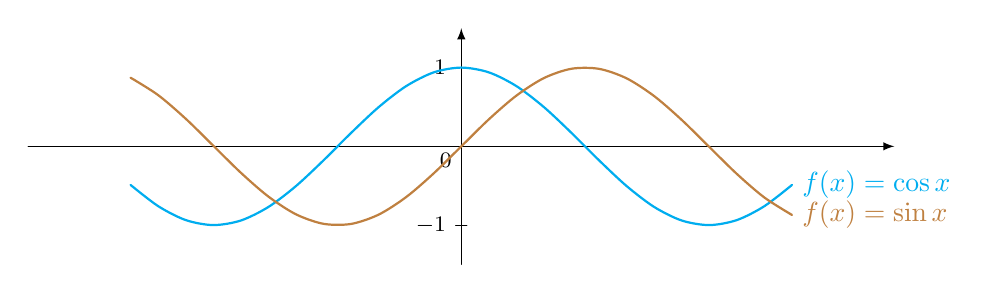
\begin{tikzpicture}[line cap=round,line join=round,]
\draw[>=latex,->,color=black] (-5.5,0) -- (5.5,0);
\foreach \x in {}
\draw[shift={(\x,0)},color=black] (0pt,2pt) -- (0pt,-2pt) node[below] {\footnotesize $\x$};
\draw[>=latex,->,color=black] (0,-1.5) -- (0,1.5);
\foreach \y in {1,-1}
\draw[shift={(0,\y)},color=black] (2pt,0pt) -- (-2pt,0pt) node[left] {\footnotesize $\y$};
\draw[color=black] (0pt,-5pt) node[left] {\footnotesize $0$};
\draw[color=cyan,smooth,thick] plot[domain=-4.2:4.2] (\x,{cos(\x r)}) node[right] {$f(x) = \cos x$};
\draw[color=brown,smooth,thick] plot[domain=-4.2:4.2] (\x,{sin(\x r)}) node[right] {$f(x) = \sin x$};
\end{tikzpicture}
%\end{tikzpicture}
\caption{نمودار دو تابع مثلثاتی $y=\sin x$ و $y=\cos x$}
\label{fig1-3}
\end{figure}

\section{انتگرال معین و نامعین و کاربرد آن در مهندسی}
در این بخش،  مفهوم انتگرال‌های معین و نامعین را توضیح داده
 و سپس خواص انتگرال معین بیان می‌شود. همچنین بعضی از کاربردهای انتگرال
 معین توضیح داده می‌شود. بعد از آن، نوبت به انتگرال‌های نامعین 
می‌رسد و روش‌های انتگرال‌گیری برای این نوع انتگرال‌ها شرح داده می‌شود.
از این روش‌ها بعدها در درس معادلات دیفرانسیل نیز استفاده می‌شود.

\subsection{انتگرال معین}
\index{انتگرال!معین}
فرض کنید $y=f(x)$ یک تابع پیوسته\index{تابع پیوسته} روی بازهٔ $[a,b]$ باشد. این بازه را به $n$ زیربازه با انتخاب $n-1$ نقطه مانند $x_1$، $x_2$، $\ldots$، $x_{n-1}$ بین $a$ و $b$ تقسیم می‌کنیم
به شرطی که 
\[
a<x_1<x_2<\cdots<x_{n-1}<b.
\]
برای ایجاد یکنواختی، $a$ را با $x_0$ و $b$ را با $x_n$ نشان می‌دهیم. شکل \ref{fig1-4} را ببینید.



\begin{theorem}[قضیه مقدار میانگین برای انتگرال‌های معین]\label{gmean}
اگر $f$ روی $[a,b]$ پیوسته باشد، آنگاه یک $c$ای در بازهٔ $[a,b]$
وجود دارد به طوری که
\[
f(c)=\dfrac{1}{b-a}\int _a ^b f(x) dx.
\]
\end{theorem}


ناحیه ممکن است  دارای شکل خاصی باشد که در این صورت، با استفاده از فرمول‌های  هندسه \cite{folland} می‌توانیم مساحت\index{مساحت} آن‌را حساب کنیم.

اگر $f$ و $g$ توابع پیوسته‌ای روی بازهٔ  $[a,b]$ و با شرط $f(x)\geq g(x)$ باشند،
آنگاه مساحت ناحیهٔ  بین منحنی‌های $y=f(x)$ و $y=g(x)$ از $a$ تا $b$ برابر است با
\begin{align}\label{ibet1}
A=\int_a^b [f(x)-g(x)] dx.
\end{align}
\subsection{منحنی‌های قاطع یکدیگر}
وقتی ناحیه‌ای توسط منحنی‌هایی که یکدیگر را قطع می‌کنند، مشخص می‌شود، 
نقاط تقاطع\index{نقاط تقاطع}، حدود انتگرال‌گیری را تعیین می‌کنند. مثال بعدی، نمونه‌ای از این 
حالت را نشان می‌دهد. در فصل بعدی باز هم نمونه‌های دیگری را بررسی خواهیم کرد که باعث فهم
بیشتر مبحث خواهد شد.


\begin{figure}[!t]
\centering
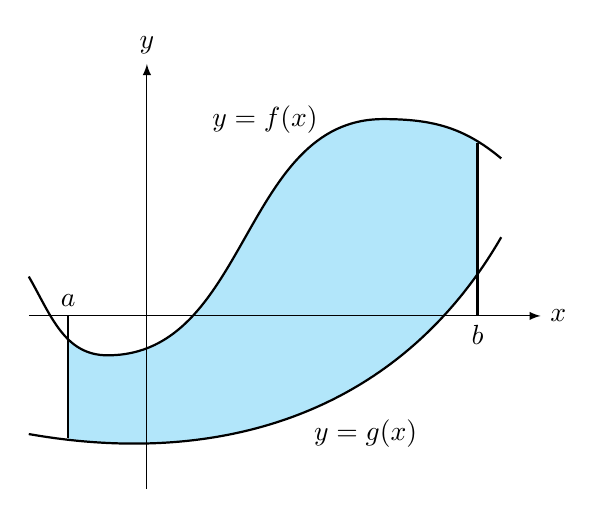
\begin{tikzpicture}[]
\begin{scope}
\clip(-1,-2)rectangle(4.2,3);
\clip (-1.5,.5) to [out=300,in=180] (-.5,-.5)
to [out=0,in=180] (3,2.5)
to [out=360,in=140] (4.5,2) --++(0,-5)--(-1,-5)--cycle;
\fill[fill=cyan,fill opacity=0.3] (-1.5,-1.5) to [out=350,in=240] (4.5,1)--++(0,5)--(-1,5)--cycle;
\end{scope}
\draw [->,>=latex] (-1.5,0) -- (5,0) node [right] {$x$};
\draw [->,>=latex] (0,-2.2) -- (0,3.2) node [above] {$y$};
\draw[thick] (-1.5,.5) to [out=300,in=180] (-.5,-.5)
to [out=0,in=180] (3,2.5)
to [out=360,in=140] (4.5,2) ;
\draw[ thick] (-1.5,-1.5) to [out=350,in=240] (4.5,1) ;
\draw[ thick] (4.2,0)--(4.2,2.2);
\node at (4.2,0) [below] {$b$};
\draw[ thick] (-1,0)--(-1,-1.55);
\node at (-1,0) [above] {$a$};
\node at (1.5,2.2) [above] {$y=f(x)$};
\node at (2,-1.5) [right] {$y=g(x)$};
\end{tikzpicture}
\caption{ناحیه محصورشده بین دو منحنی $y=f(x)$ و $y=g(x)$}
\label{fig1-4}
\end{figure}

با توجه به شکل، طول قطعه‌خط خاص $PQ$ برابر 
$L$
است. بنابراین طول منحنی به وسیلهٔ جمع 
\[
\sum_{k=1}^{n}\sqrt{(\Delta x_k)^2+(\Delta y_k)^2}
\]
تقریب زده می‌شود. 

\begin{premind}[محاسبه مشتق]
اگر $x_1$ عدد خاصی از دامنهٔ $f$ باشد، آنگاه می‌توان نوشت
\begin{align}\label{bderi2}
f'(x_1)=\lim_{\Delta x\rightarrow 0}\dfrac{f(x_1+\Delta x) - f(x_1)}{\Delta x}
\end{align}
البته به شرطی که این حد وجود داشته باشد. از رابطهٔ \eqref{bderi2} برای محاسبهٔ مشتق تابع $f$ در یک نقطهٔ 
خاص مانند $x_1$ استفاده می‌شود. 

اگر در رابطهٔ \eqref{bderi2} قرار دهیم $x_1+\Delta x=x$، آنگاه عبارت
 «$\Delta x\rightarrow 0$» 
معادل «$x\rightarrow x_1$»
است. بنابراین با توجه به فرمول \eqref{bderi2} می‌توان نوشت
\begin{align*}
f'(x_1)=\lim_{ x\rightarrow x_1}\dfrac{f(x) - f(x_1)}{x-x_1}
\end{align*}

تابع $f$ را در $x_1$ مشتق‌پذیر گوییم، اگر $f'(x_1)$ وجود داشته باشد.
تابع $f$ را روی بازهٔ $I$ مشتق‌پذیر گوییم، اگر $f$ به ازای هر عدد واقع در این بازه، مشتق‌پذیر باشد.
\end{premind}
\begin{example}
مساحت ناحیهٔ محصور ایجاد شده توسط سهمی $y=2-x^2$ و خط $y=-x$ را پیدا
کنید.
\end{example}
%\endinput

\begin{solution}
ابتدا نمودار\index{نمودار منحنی} هر دو منحنی را رسم می‌کنیم (شکل \ref{fig1-6}). 
 طبق رابطهٔ \eqref{ibet1}، قرار می‌دهیم
$f(x)=2-x^2$
و
$g(x)=-x$.
حال برای پیدا کردن حدود انتگرال‌گیری\index{حدود انتگرال‌گیری}، معادلهٔ $2-x^2=-x$ را حل می‌کنیم. بنابراین
$x^2-x-2=0$.
لذا
%\[(x+1)(x-2)=0\]
%که نتیجه می‌شود که
%\bal*
%f(x)-g(x)&= (2-x^2)-(-x)\\
%&=2-x^2+x\\
%&=2+x-x^2.
%\eal
%حال
 می‌توان نوشت
\begin{align*}
A&=\int_a^b [f(x)-g(x)]dx\\[2mm]
&=\int_{-1}^{2}(2+x-x^2)dx\\[2mm]
&=\Bigg[2x+\dfrac{x^2}{2}-\dfrac{x^3}{3}\Bigg]_{-1}^{2}\\[2mm]
&=\Big(4+\dfrac{4}{2}-\dfrac{8}{3}\Big)-\Big(-2+\dfrac{1}{2}+\dfrac{1}{3}\Big)%\\[2mm]
\end{align*}
که کار را تمام می‌کند.
\end{solution}
\threecolumnfootnotes
این ایده‌ها برای اولین بار توسط صاحب ‌جهرمی\LTRfootnote{Saheb-Djahromi} و کازن\LTRfootnote{Lepoldo Smith Kozen}
مطرح شد. هنگامی که کازن با فضاهای اندازه مطلق کار می‌کرد، اندازه‌های (احتمال) در نظر گرفته شده قبلی، به وسیله مجموعه‌های اسکات-باز یک \lr{dcpo} گسترش پیدا کرد.

 این ارتباط بین محاسبه‌پذیری و توپولوژی، بطور بسیار واضح توسط اسمیت\LTRfootnote{George Smyth}  شرح داده شده و  بعدها توسط آبرامسکی\LTRfootnote{Abramsky}، ویکرز\LTRfootnote{John Vickers} و دیگران، بیشتر توسعه داده شد.

روش گفته شده در بالا، روش دیسک\index{روش!دیسک} (شکل \ref{fig1-6}) نام دارد. روش دیگری نیز برای محاسبهٔ
حجم حاصل از دوران وجود دارد که به روش واشر\index{روش!واشر}، معروف شده است . در ادامه بیشتر با این روش آشنا خواهیم شد.%
\cite{vahid90}

\begin{figure}[]
\centering
\begin{tikzpicture}[line cap=round,line join=round,>=triangle 45,x=1.0cm,y=1.0cm,]
\draw[->,>=latex,color=black] (-0.5,0) -- (5.5,0);
\draw[->,>=latex,color=black] (0,-0.5) -- (0,5);
\draw[color=black] (0pt,-5pt) node[left] {\footnotesize $0$};
\draw[thick,cyan] (2,.5) to [out=80,in=270] (1.5,2)
to [out=90,in=220] (3,4);
\draw[thick,cyan] (3,.5) to [out=80,in=255] (3.5,2.2)
to [out=80,in=330] (2,4.5);
\draw[thick,dashed] (0,1) -- (3.1,1);
\node at (0,3.9) [left] {\small $d$};
\draw[thick,dashed,] (0,3.9) -- (2.9,3.9);
\node at (0,1) [left] {\small $c$};
\node at (3.5,2.5) [right] {\small $x=f(y)$};
\node at (1.6,2.5) [left] {\small $x=g(y)$};
\node at (5.5,0) [right] {\small $x$};
\node at (0,5) [above] {\small $y$};
\end{tikzpicture}
\caption{نمودار منحنی‌های 
 $x=g(y)$ و $x=f(y)$
 در بازه $[c,d]$}
\label{fig1-6}
\end{figure}
\begin{pdefinition1}[روش واشر]\label{defi4}
هرگاه ناحیه‌ای که برای تولید یک جسم، دوران داده می‌شود، محور دوران را قطع نکند، جسم تولید شده، دارای یک سوراخ خواهد بود. در این روش، از فرمول
\begin{align}\label{10eq3}
V=\int_a^b \pi ([R(x)]^2-[r(x)]^2)\di x
\end{align}
استفاده می‌شود که در آن، $R(x)$ 
شعاع بیرونی\index{شعاع!بیرونی واشر در دوران}
 و
 $r(x)$
 شعاع داخلی واشر\index{شعاع!داخلی واشر در دوران}
 است. 
\end{pdefinition1}
دقت داشته باشید که در فرمول \eqref{10eq3} اگر $r(x)$ در سراسر بازهٔ
$[a,b]$ 
صفر باشد، همان فرمول روش دیسک، نتیجه می‌شود. بنابراین روش دیسک، حالت خاصی از روش واشر است.
 
سوالی که ممکن است در اینجا پیش بیاید این است که کدام‌یک از ۳ روش گفته شده، بهتر است؟ واقعیت این است که به طور قطع، نمی‌توان گفت که کدام روش، همیشه بهتر از بقیه عمل می‌کند.
% بنابراین در هر مساله، باید ابتدا
%ناحیه مورد نظر را رسم کرده و سپس با توجه به آن، بهترین روش را انتخاب کنیم.
جسم‌های حاصل از دوران\index{جسم حاصل از دوران}، جسم‌هایی هستند که شکل آن‌ها از دوران\index{دوران} حول محور‌ها به دست می‌آید. 
%گاهی جسم‌های تولید شده، جسم‌هایی هستند که با استفاده از فرمول‌های هندسه، به راحتی می‌توانیم حجم آن‌ها را حساب کنیم؛ بنابراین
\begin{align*}
V=\int_c^d\pi ([R(y)]^2-[r(y)]^2)\di y+
\int_0^1\pi \Big(\Big[\dfrac{3}{2}-\sqrt{y}\Big]^2\Big)\di y.
\end{align*}

\begin{figure}
\centering
\subfloat[][ناحیهٔ محصور ایجاد شده توسط سهمی $y=2-x^2$ و خط $y=-x$
]{
\begin{tikzpicture}[line cap=round,line join=round,>=triangle 45,x=1.0cm,y=1.0cm,]
\draw[->,>=latex,color=black] (-1.5,0) -- (3.5,0);
\foreach \x in {-1,-1,1,2,3}
\draw[shift={(\x,0)},color=black] (0pt,2pt) -- (0pt,-2pt) node[below] {\footnotesize $\x$};
\draw[->,>=latex,color=black] (0,-2.5) -- (0,3);
\foreach \y in {-2,-1,1,2,2.5}
\draw[shift={(0,\y)},color=black] (2pt,0pt) -- (-2pt,0pt);
\draw[color=black] (0pt,-1pt) node[below left] {\footnotesize $0$};
\node at (-1,1) [left ] {\small $(-1,1)$};
\node at (3.5,0) [right ] {\small $x$};
\node at (0,3) [above ] {\small $y$};
\clip[] (-1.5,-2.5) rectangle (3.5,3);
\draw [thick,domain=-1.5:2.5] plot(\x,{-1*(\x)});
\draw [smooth,  thick,domain=-2:3] plot(\x,{-1*(\x)^2+2});
\node at (2,-2) [right] {\small $(2,-2)$};
\node at (.7,-1.2) [below ] {\small $y=-x$};
\node at (1,1) [right ] {\small $y=2-x^2$};
\draw [fill=cyan,fill opacity=0.3] plot [domain=-1:2](\x,{-1*(\x)^2+2}) -- plot [domain=-2:3] (\x,{-1*(\x)});
\end{tikzpicture}
\label{subfig1}}
\subfloat[][نمودار تابع  $y=({x}/{2})^{2/3}$ در بازه $I$]{
\begin{tikzpicture}[line cap=round,line join=round,>=triangle 45,x=2cm,y=2cm,]
\draw[>=latex,->,color=black] (-.2,0) -- (2.3,0);
\foreach \x in {1,2}
\draw[shift={(\x,0)},color=black] (0pt,2pt) -- (0pt,-2pt) node[below] {\footnotesize $\x$};
\draw[>=latex,->,color=black] (0,-0.3) -- (0,2.4);
\foreach \y in {1}
\draw[shift={(0,\y)},color=black] (2pt,0pt) -- (-2pt,0pt) node[left] {\footnotesize $\y$};
\draw[color=black] (0pt,-5pt) node[left] {\footnotesize $0$};
\node at (.8,1.1) [below] { $y=\Big(\dfrac{x}{2}\Big)^{2/3}$};
\node at (2,.95) [ below] { $(2,1)$};
\node at (2.3,0) [right] {\small $x$};
\node at (0,2.4) [above] {\small $y$};
\draw[cyan,thick, smooth,samples=5.5*\sqrtsamples,domain=0.001:2]plot(\x,{exp(2*ln(\x/2)/3)});
\draw [fill=cyan](2,1) circle (.7mm);
\end{tikzpicture}
\label{subfig2}}

\caption{نمودار تعریف \ref{defi4} در حالت متقارن}

\end{figure}

\section{محاسبهٔ طول منحنی‌ها با روشی ابتکاری}\index{طول منحنی}
فرض کنید می‌خواهیم طول منحنی $y=f(x)$ را از $x=a$ تا $x=b$ پیدا کنیم.
طبق معمول، بازهٔ $[a,b]$ را افراز\index{افراز} می‌کنیم و نقاط متناظر روی منحنی را با قطعه‌خط‌هایی به همدیگر وصل می‌کنیم تا یک مسیر چندضلعی تشکیل شود (شکل \ref{fig1-8}).


%\begin{figure}
%\centering
%\begin{tikzpicture}[]
%     \draw [->,>=latex] (-1,1) -- (8,1) node [right] {$x$};
%     \draw [->,>=latex] (-.5,.5) -- (-.5,5.5) node [above] {$y$};
%     \node at (-.5,1) [below left] {$0$};
%
%\draw[very thick,cyan] (1,4) to [out=0,in=180] (4,2)
%to [out=0,in=180] (7,5);
%\node at (1,4) [left] {$A$};
%\node at (1,1) [below] {$a$};
%\node at (4,2) [below left] {$P$};
%\node at (4,1) [below ] {$x_{k-1}$};
%\draw[dashed, thick] (1,4) -- (1,1);
%\draw[dashed, thick] (5.5,2) -- (5.5,1);
%\draw[dashed, thick] (4,2) -- (4,1);
%\draw[dashed, thick] (7,5) -- (7,1);
% \node at (7,5) [right ] {$B$};
% \node at (5.5,3.5) [right ] {$Q$};
%\draw[thick] (4,2) -- (5.5,2) ;
%\draw[thick] (5.5,2) -- (5.5,3.5) ;
%\draw[] (4.7,2.9) -- (4,3.5) ;
% \node at (3.8,3.5) [above ] {$\sqrt{(\Delta x_k)^2+(\Delta y_k)^2}$};
% \node at (4.75,2) [below ] {$\Delta x_k$};
% \node at (5.5,2.75) [right ] {$\Delta y_k$};
% \node at (7,1) [below ] {$b$};
% \node at (5.5,1) [below ] {$x_k$};
%\draw[ thick] (1,4) -- (4,2);
%\draw[ thick] (4,2) -- (7,5);
%\end{tikzpicture}
%\caption{
%مسیر چندضلعی پوشاننده طول منحنی $y=f(x)$  از نقطه $A$ تا نقطه $B$
%} 
%\label{fig1-7}
%\end{figure}
\begin{pdefinition1}
اگر $f$ روی بازهٔ $[a,b]$ هموار باشد، طول منحنی $y=f(x)$ از $a$ تا $b$ برابر است با
\begin{align}\label{10eq6}
L=\int_a^b \sqrt{1+\Big(\dfrac{dy}{dx}\Big)^2}\di x=\int_a^b \sqrt{1+(f'(x))^2}\di x.
\psymbol{$L$}{طول منحنی}
\end{align}
\end{pdefinition1}
گاهی ممکن است $dy/dx$ در یک نقطهٔ خاص از بازهٔ انتگرال‌گیری موجود 
نباشد. در این حالت
$dx/dy$
را حساب می‌کنیم و $x$ را بر حسب تابعی از $y$ بیان می‌کنیم (شکل \ref{fig1-8}).

\begin{figure}[!h]
\centering
\begin{tikzpicture}[line cap=round,line join=round,>=triangle 45,x=1cm,y=1cm]
\draw[->,>=latex,color=black] (-0.5,0) -- (2.5,0);
\foreach \x in {1}
\draw[shift={(\x,0)},color=black] (0pt,2pt) -- (0pt,-2pt) node[below] {\small $\x$};
\draw[->,>=latex,color=black] (0,-.5) -- (0,3);
\foreach \y in {1}
\draw[shift={(0,\y)},color=black] (2pt,0pt) -- (-2pt,0pt) node[left] {\small $\y$};
\draw[color=black] (0pt,-5pt) node[left] { $0$};
\node at (2.5,0) [right] {\small $x$};
\node at (0,3) [above] {\small $y$};
\node at (.5,1.7) [right] {\small $y=\dfrac{1}{\sqrt{x}}$};
\clip(0,0) rectangle (1,2.5);
\draw[thick, smooth,samples=5.5*\sqrtsamples,domain=0.001:1] 
plot(\x,{1/sqrt((\x))});
\fill [cyan,fill opacity=0.3] plot [samples=5.5*\sqrtsamples,domain=0.001:1](\x,{1/sqrt((\x))})-- (1,0)--
(0,0);
\end{tikzpicture} 
\caption{
نمونه‌ای از تابعی با برد نامعین 
}
\label{fig1-8}
\end{figure}

\section{انتگرال‌های ناسره}
انتگرال‌های معینی که تا اینجا با آن‌ها سر و کار داشته‌ایم، دارای دو ویژگی بوده‌اند.%
\cite{aliprantis}
یکی اینکه، دامنهٔ انتگرال‌گیری آن‌ها، یعنی $a$ و $b$ معین بود. دوم اینکه، برد
انتگرالده\index{انتگرالده} روی این دامنه، معین بود. در این بخش یاد 
می‌گیریم که چگونه باید با این انتگرال‌ها برخورد کنیم  (جدول \ref{tab1-1}).
\begin{example}
همگرایی 
\[
\int_{0}^{3}\dfrac{dx}{(x-1)^{2/3}}
\]
را بررسی کنید.
\end{example}

\begin{solution}
انتگرالده $f(x)=1/(x-1)^{2/3}$ در $x=1$ نامتناهی می‌شود؛  اما 
روی $[0,1)$ و $(1,3]$ پیوسته است.
همگرایی انتگرال روی $[0,3]$ به انتگرال‌های از $0$ تا $1$ و $1$ تا $3$ بستگی
دارد. روی $[0,1]$ داریم

\begin{align*}
\int_{0}^{1}\dfrac{dx}{(x-1)^{2/3}}&=
	\lim_{b\rightarrow 1^{-}}\int_{0}^{b}\dfrac{dx}{(x-1)^{2/3}}\\[3mm]
	&=\lim_{b\rightarrow 1^{-}}[3(b-1)^{1/3}-3(0-1)^{1/3}]\\
	&=3
\end{align*}
و لذا نتیجه به دست می‌آید.
\end{solution}

\section{محاسبهٔ حجم جسم‌های حاصل از دوران}
جسم‌های حاصل از دوران، جسم‌هایی هستند که شکل آن‌ها از دوران حول محور‌ها به دست می‌آید. گاهی جسم‌های تولید شده، جسم‌هایی هستند که با استفاده از فرمول‌های هندسه، به راحتی می‌توانیم حجم آن‌ها را حساب کنیم؛ اما گاهی شکل این جسم‌ها، منظم نیست و لذا ناچاریم برای محاسبهٔ حجم آن‌ها از حساب دیفرانسیل\index{حساب دیفرانسیل} و انتگرال کمک بگیریم. 
در ادامه دربارهٔ حجم این نوع جسم‌ها بحث می‌کنیم.

\begin{table}[!t]
\centering
\caption{
نحوه عملکرد تابع $f$ در ارتباط با پیوستگی
}
\begin{tabular}{ccc}
\toprule
نام تابع & نقطه ناپیوستگی & نقطه بحرانی
\\
\midrule
تابع $f$ & 
$x=1$ & $a^2+3$\\
تابع $g$ & 
$x=-2$ & $b-4$\\
تابع $h$ & 
$x=0$ & $a+b-7$
\\ \bottomrule
\end{tabular}
\label{tab1-1}
\end{table}
\subsection{حجم حاصل از دوران حول محور $x$ها}
حجم جسم حاصل از دوران ناحیهٔ بین محور $x$ها و  نمودار تابع پیوستهٔ $y=R(x)$،
$a\leq x\leq b$
 حول محور $x$ها برابر است با
 \begin{align}\label{10eq1}
 V=\int_a^b \pi (R(x))^2 \di x
 \end{align}
  این 
ناحیه ممکن است  دارای شکل خاصی باشد که در این صورت، با استفاده از فرمول‌های  هندسه می‌توانیم مساحت آن‌را حساب کنیم؛ اما اگر $f$ و $g$ توابع پیوستهٔ 
دلخواهی باشند، ناچاریم که مساحت مورد نظر را با استفاده از انتگرال حساب کنیم. 
 حال می‌توان کد این رابطه را به صورت زیر نوشت.
\begin{lstlisting}[caption={محاسبه حجم جسم حاصل از دوران},
label={code1}
]  
\def\@makechapterhead#1{%
  \vspace*{50\p@}%
  {\parindent \z@ \raggedright \normalfont
    \ifnum \c@secnumdepth >\m@ne
      \if@mainmatter
        \huge\bfseries \@chapapp\space \thechapter
        \par\nobreak
        \vskip 20\p@
      \fi
    \fi
   \interlinepenalty\@M
  \Huge \bfseries #1\par\nobreak
 \vskip 40\p@
}}                                           
\end{lstlisting} 
\subsection{حجم حاصل از دوران حول محور $y$ها}
حجم جسم حاصل از دوران\index{جسم حاصل از دوران} ناحیهٔ بین محور $y$ها و  نمودار تابع پیوستهٔ\index{تابع پیوسته} $x=R(y)$،
$c\leq y\leq d$
 حول محور $y$ها برابر است با
 \begin{align}\label{10eq2}
 V=\int_c^d \pi (R(y))^2 dy
 \end{align}

 حال اگر بتوانیم فرمولی برای طول مسیر ایجاد شده بیابیم، آنگاه فرمولی برای تقریب طول منحنی $AB$ نیز خواهیم داشت. 


 
 
\begin{example}
مساحت ناحیه‌ای در ربع اول که از بالا به $y=\sqrt{x}$ و از پایین به محور $x$ها
و خط $y=x-2$ محدود است را بیابید. 
\end{example}

\begin{solution}
ابتدا نمودار هر دو تابع را رسم می‌کنیم.
با توجه به شکل بالا، 
مرز سمت راستی ناحیه، خط $x=y+2$ است.  گاهی جسم‌های تولید شده، جسم‌هایی هستند که با استفاده از فرمول‌های هندسه، به راحتی می‌توانیم حجم آن‌ها را حساب کنیم؛ 
لذا $f(y)=y+2$ است و مرز 
$y=-1$ و $y=2$ 
است.
حال چون، مقدار $y=-1$، یک نقطهٔ تقاطع پایین محور $x$ها را به دست 
می‌دهد، لذا قابل قبول نیست. بنابراین فقط مقدار $y=2$ قابل قبول بوده و لذا
$b=2$ 
است. 
\begin{figure}[!t]
\centering
\includegraphics[width=\textwidth]{nash}
\caption{
جان نش در کلاس درس
}\label{nash}
\end{figure}

حال از رابطهٔ بالا استفاده می‌کنیم.
\begin{align*}
A=\int_c^d [f(y)-g(y)] dy&=\int_0^2[2+y-y^2] dy\\[2mm]
&=\Bigg[2y+\dfrac{y^2}{2}-\dfrac{y^3}{3}\Bigg]_{0}^{2}\\[2mm]
%&=4+\dfrac{4}{2}-\dfrac{8}{3}\\[2mm]
&=\dfrac{10}{3}.
\end{align*}

بنابراین $A=10/3$ است. 
\end{solution}
هرگاه ناحیه‌ای که برای تولید یک جسم، دوران داده می‌شود، محور دوران را قطع نکند، جسم تولید شده، دارای یک سوراخ خواهد بود. در این روش، از فرمول
\begin{align}\label{10eq3}
V=\int_a^b \pi ([R(x)]^2-[r(x)]^2)\di x
\end{align}
استفاده می‌شود که در آن، $R(x)$ 
شعاع بیرونی\index{شعاع!بیرونی واشر در دوران}
 و
 $r(x)$
 شعاع داخلی واشر\index{شعاع!داخلی واشر در دوران}
 است. 
 
همان‌طور که دیده می‌شود، نتیجهٔ به دست آمده، با نتیجهٔ مثال قبل
یکسان است و با مقدار محاسبات کمتری به دست آمده است. همچنین دقت شود که در این مثال، چون نسبت به $y$ انتگرال گرفته‌ایم، تنها یک 
انتگرال‌گیری لازم است. 
 

\section{قواعد انتگرال‌گیری نامعین}\index{انتگرال!نامعین}
حجم جسم حاصل از دوران ناحیهٔ بین محور $x$ها و  نمودار تابع پیوستهٔ $y=R(x)$،
$a\leq x\leq b$
 حول محور $x$ها برابر است با
 \begin{align}\label{c2eq1}
 V=\int_a^b \pi (R(x))^2 \di x
 \end{align}
\begin{example}
ناحیهٔ بین منحنی $y=\sqrt{x}$، 
$0\leq x\leq 4$
و محور $x$ها، برای تولید جسمی، حول محور $x$ها دوران داده می‌شود. حجم آن‌‌را
را پیدا کنید.
\end{example}
حجم جسم حاصل از دوران\index{جسم حاصل از دوران} ناحیهٔ بین محور $y$ها و  نمودار تابع پیوستهٔ\index{تابع پیوسته} $x=R(y)$،
$c\leq y\leq d$
 حول محور $y$ها برابر است با
 \begin{align}\label{c2eq2}
 V=\int_c^d \pi (R(y))^2 \di y
 \end{align}
\section{تکنیک‌های انتگرال‌گیری}
\subsection{انتگرال‌گیری جزء به جزء}\index{روش!انتگرال‌گیری جزء به جزء}
انتگرال‌گیری جزء به جزء یکی از تکنیک‌هایی است که برای ساده کردن انتگرال‌هایی به فرم
\begin{align}
\int f(x) g(x) dx
\end{align}
به کار می‌رود؛ به شرطی که در آن، از  $f$ بتوان بارها مشتق گرفت و از $g$ نیز بتوان به سادگی، انتگرال گرفت. انتگرال 
\[
\int xe^x dx,
\]
یک نمونه از چنین انتگرالی است؛ زیرا از  $f(x)=x$ می‌توان دو بار مشتق گرفت تا صفر شود و از 
$g(x)=e^x$
نیز می‌توان به سادگی، بارها انتگرال گرفت. انتگرال‌گیری جزء به جزء، همچنین برای انتگرال‌هایی
مانند 
\[
\int e^x \sin x dx
\]
که در آن‌ها، هر قسمت از انتگرالده بعد از مشتق‌گیری و یا انتگرال‌گیری مکرر، دوباره تکرار می‌شوند، نیز به کار می‌رود. 

\subsection{جانشینی ساده‌کننده}\index{روش!جانشینی ساده‌کننده}
گوییم تابع $F(x)$ یک ضدمشتق تابع $f(x)$ است، هر گاه برای هر $x$ در
دامنهٔ $f$ داشته باشیم
\[
F'(x)=f(x).
\]
مجموعهٔ تمام ضدمشتق‌های $f$، انتگرال نامعین $f$ نسبت به
$x$
نامیده شده و با علامت
\[
\int f(x) dx
\]
نشان داده می‌شود.
\subsection{کسرهای جزیی}\index{روش!جانشینی ساده‌کننده}
طبق قضیهٔ مقدار میانگین، می‌دانیم توابعِ با مشتق یکسان، در یک عدد ثابت
 با یکدیگر اختلاف دارند. به عبارت دیگر، اگر  دو تابع $f$ و $g$، مشتق یکسانی داشته باشند، آنگاه $f(x)=g(x)+C$ است. بنابراین می‌توان نتیجه 
 گرفت که هر گاه یک ضدمشتق $F$ برای تابع $f$ پیدا کنیم، ضدمشتق‌های دیگر $f$ در یک ثابت، با $F$ تفاوت دارند.
 می‌توان نتیجه 
 گرفت که هر گاه یک ضدمشتق $F$ برای تابع $f$ پیدا کنیم، ضدمشتق‌های دیگر $f$ در یک ثابت، با $F$ تفاوت دارند. این حالت را در انتگرال‌گیری با 
\[
 \int f(x)dx= F(x)+C
\]
 نشان می‌دهیم.
\section{ظاهر شدن انتگرال اصلی در فرایند انتگرال‌گیری}
در این بخش چند حکم را با هم مرور می‌کنیم. 
\begin{lemma}
مقدار  $\int_0 ^1\sqrt{1+\cos x} dx $ نمی‌تواند ۲ باشد.
\end{lemma}
\begin{proof}
به دلیل سادگی برهان، به عنوان تمرین به خواننده واگذار می‌شود.
\end{proof}
\begin{proposition}
مقدار  $\int_0 ^1\sqrt{1+\cos x} dx $ نمی‌تواند ۲ باشد.
\end{proposition}
\begin{corollary}
مقدار  $\int_0 ^1\sqrt{1+\cos x} dx $ نمی‌تواند ۲ باشد.
\end{corollary}
\begin{remark}
مقدار  $\int_0 ^1\sqrt{1+\cos x} dx $ نمی‌تواند ۲ باشد.
\end{remark}





اگر  $f(x)=3x^2+12$ باشد، مشتق آن‌را حساب کنید.
اگر $x$ عددی در دامنهٔ $f$ باشد، با استفاده از مطالب قبلی داریم
\begin{align*}
f'(x)&=\lim_{\Delta x\rightarrow 0}\dfrac{f(x+\Delta x) - f(x)}{\Delta x}\\[2mm]
&=\lim_{\Delta x\rightarrow 0}\dfrac{3(x+\Delta x)^{2}+12 - (3x^2+12)}{\Delta x}\\[2mm]
&=\lim_{\Delta x\rightarrow 0}\dfrac{3x^2+6x\Delta x+3(\Delta x)^{2}+12-3x^2-12}{\Delta x}\\[2mm]
&=\lim_{\Delta x\rightarrow 0}\dfrac{6x\Delta x+3(\Delta x)^{2}}{\Delta x}\\[2mm]
&=\lim_{\Delta x\rightarrow 0}6x+3(\Delta x)\\[2mm]
&=6x
\end{align*}
و لذا مشتق تابع $f$ به دست می‌آید.
اگر $x_1$ عدد خاصی از دامنهٔ $f$ باشد، آنگاه می‌توان نوشت
\begin{align}\label{c2deri2}
f'(x_1)=\lim_{\Delta x\rightarrow 0}\dfrac{f(x_1+\Delta x) - f(x_1)}{\Delta x}
\end{align}
البته به شرطی که این حد وجود داشته باشد. از رابطهٔ \eqref{c2eri2} برای محاسبهٔ مشتق تابع $f$ در یک نقطهٔ 
خاص مانند $x_1$ استفاده می‌شود. 

اگر در رابطهٔ \eqref{c2deri2} قرار دهیم $x_1+\Delta x=x$، آنگاه عبارت
 «$\Delta x\rightarrow 0$» 
معادل «$x\rightarrow x_1$»
است. بنابراین با توجه به فرمول \eqref{bderi2} می‌توان نوشت
\begin{align}\label{c2deri3}
f'(x_1)=\lim_{ x\rightarrow x_1}\dfrac{f(x) - f(x_1)}{x-x_1}
\end{align}
مشتق تابع $f(x)=3x^2+12$ را در نقطهٔ $x=2$ حساب کنید.

و لذا مشتق تابع $f$ در نقطهٔ $x=2$ به دست می‌آید.
تابع $f$ را در $x_1$ مشتق‌پذیر گوییم، اگر $f'(x_1)$ وجود داشته باشد.
تابع $f$ را روی بازهٔ $I$ مشتق‌پذیر گوییم، اگر $f$ به ازای هر عدد واقع در این بازه، مشتق‌پذیر باشد.
اگر $f(x)=3x^2+12$ باشد، تعیین کنید که $f$ در کجا مشتق‌پذیر است؟
از آنجایی که $f'(x)=6x$  و $6x$ برای تمام اعداد حقیقی موجود است، لذا نتیجه
می‌شود که $f$ در همه جا مشتق‌پذیر است.
اگر تابع $f$ در $x_1$ تعریف شده باشد، آنگاه مشتق راست $f$ در $x_1$ با $f'_{+}(x_1)$ نشان داده
می‌شود و به صورت 
\begin{align}
f'_{+}(x_1)=\lim_{\Delta x\rightarrow 0^{+}}\dfrac{f(x_1+\Delta x) - f(x_1)}{\Delta x}
\end{align}
و یا به عبارت دیگر،
\begin{align}
f'_{+}(x_1)=\lim_{ x\rightarrow x_1^{+}}\dfrac{f(x) - f(x_1)}{x-x_1}
\end{align}
تعریف می‌شود؛ به شرطی که این حدود موجود باشند.
اگر تابع $f$ در $x_1$ تعریف شده باشد، آنگاه مشتق چپ $f$ در $x_1$ با $f'_{-}(x_1)$ نشان داده
می‌شود و به صورت 
\begin{align}
f'_{-}(x_1)=\lim_{\Delta x\rightarrow 0^{-}}\dfrac{f(x_1+\Delta x) - f(x_1)}{\Delta x}
\end{align}
و یا به عبارت دیگر،
\begin{align}
f'_{-}(x_1)=\lim_{ x\rightarrow x_1^{-}}\dfrac{f(x) - f(x_1)}{x-x_1}
\end{align}
تعریف می‌شود؛ به شرطی که این حدود موجود باشند.
فرض کنید تابع $f$ به صورت 
\[
f(x)=\left\{\begin{array}{ll}
2x-1& x<3\\
8-x & 3\leq x
\end{array} \right.
\]
تعریف شده است. پیوستگی و مشتق‌پذیری این تابع را در نقطهٔ $x=3$ بررسی کنید.
برای بررسی پیوستگی، سه شرط پیوستگی را بررسی می‌کنیم. (۱) داریم $f(3)=5$. بنابراین شرط اول که همان
موجود بودن $f(3)$ است، برقرار است. (۲) برای بررسی شرط دوم داریم
\[
\lim _{x\rightarrow 3^{-}}f(x)=\lim_{x\rightarrow 3^{-}} (2x-1)=5
\]
و 
\[
\lim _{x\rightarrow 3^{+}}f(x)=\lim_{x\rightarrow 3^{+}} (8-x)=5.
\]
بنابراین
 $\lim_{x\rightarrow 3}f(x)=5$
و لذا شرط دوم هم برقرار است. (۳)
$\lim_{x\rightarrow 3}f(x)=f(3)$.
بنابراین $f$ در $3$ پیوسته است. حال مشتق‌پذیری $f$ را در $3$ بررسی می‌کنیم. داریم
\begin{align*}
f'_{-}(3)&=\lim_{\Delta x\rightarrow 0^{-}}\dfrac{f(3+\Delta x)-f(3)}{\Delta x}\\
&=\lim_{\Delta x\rightarrow 0^{-}}\dfrac{(2(3+\Delta x)-1)-5}{\Delta x}\\
&=\lim_{\Delta x\rightarrow 0^{-}}\dfrac{6+2\Delta x-6}{\Delta x}\\
%&=\lim_{\Delta x\rightarrow 0^{-}} 2\\
&=2.
\end{align*}

\section{سه جانشینی بنیادی}
تابع $f$ را در $x_1$ مشتق‌پذیر گوییم، اگر $f'(x_1)$ وجود داشته باشد.
تابع $f$ را روی بازهٔ $I$ مشتق‌پذیر گوییم، اگر $f$ به ازای هر عدد واقع در این بازه، مشتق‌پذیر باشد.

جان اسمیت در کتابش می‌نویسد:
\begin{pquote}
طبق قضیهٔ مقدار میانگین، می‌دانیم توابعِ با مشتق یکسان، در یک عدد ثابت
 با یکدیگر اختلاف دارند. به عبارت دیگر، اگر  دو تابع $f$ و $g$، مشتق یکسانی داشته باشند، آنگاه $f(x)=g(x)+C$ است. بنابراین می‌توان نتیجه 
 گرفت که هر گاه یک ضدمشتق $F$ برای تابع $f$ پیدا کنیم، ضدمشتق‌های دیگر $f$ در یک ثابت، با $F$ تفاوت دارند.
\end{pquote}
فرض کنید می‌خواهیم طول منحنی $y=f(x)$ را از $x=a$ تا $x=b$ پیدا کنیم.
طبق معمول، بازهٔ $[a,b]$ را افراز\index{افراز} می‌کنیم و نقاط متناظر روی منحنی را با قطعه‌خط‌هایی به همدیگر وصل می‌کنیم تا یک مسیر چندضلعی تشکیل شود.


\index{تابع!اکیداً نزولی}
\index{تابع!اکیداً صعودی}
\index{هم‌پوشانی}
\index{هم‌پیمانه}
\index{لاپلاس}
\index{لاگرانژ}
\index{حجم جسم حاصل از دوران}
\index{شعاع!بیرونی واشر در دوران}
\index{لژاندر}
\index{عملگر}
\index{عملگر!خطی}
\index{هم‌پیوستگی}
\index{حرکت پرتابه}
\index{چینش}
\index{دلتا}
\index{ردیف}
\index{ویرایش}
\index{وارون تابع}
\index{واژگونی}
\index{گشتاور}
\index{گرانش}
\index{گرادیان}
\index{دیورژانس}
\index{زاویه فاز}
\index{مشتق!جهتی}
\index{مثلث}
\index{روش!رادیکالی}
\index{زتا}
\index{دوران}
\index{نپر}
\index{تابع}
\index{اکید}
 


\begin{pproblems}[تمرین‌ها]
\item \label{p1-1}
اگر  $f(x)=3x^2+12$ باشد، مشتق آن‌را حساب کنید.
\item \label{p1-2}
نشان دهید مقدار 
\[
\int_0 ^1\sqrt{1+\cos x} dx
\]
نمی‌تواند ۲ باشد.
\item \label{p1-3}
از نامساوی 
$\cos x\geq (1-x^2/2)$
که برای هر $x$ی برقرار است، استفاده کنید و یک کران پایین برای مقدار 
$\int _0 ^1 \cos x  dx$
پیدا کنید.
\item \label{p1-4}
مشتق تابع $f(x)=3x^2+12$ را در نقطهٔ $x=2$ حساب کنید.
\item \label{p1-5}
اگر $f(x)=3x^2+12$ باشد، تعیین کنید که $f$ در کجا مشتق‌پذیر است؟
\item \label{p1-6}
متحرکی روی نمودار $y=\sqrt{x-2}$ با فرض $x\geq 2$ حرکت می‌کند. اگر مؤلفهٔ $x$ آن با آهنگ $2$ متر بر ثانیه
افزایش یابد، در لحظه‌ای که $x=6$ است، آهنگ تغییر مؤلفه $y$ آن برابر چیست؟ آیا متحرک در حال صعود است یا نزول؟
\item \label{p1-7}
مشتق تابع 
$y=(\sqrt{x}+1)(\sqrt{x}-1)(x+1)$
را حساب کنید.
\item \label{p1-8}
مشتق 
\[
f(x)=\dfrac{(x-1)(x^2-2x)}{x^4}
\]
را حساب کنید. 
\item \label{p1-9}
طول منحنی زیر را چطور می‌توان محاسبه کرد؟
\begin{center}
\begin{tikzpicture}[line cap=round,line join=round,>=triangle 45,x=1cm,y=1cm]
\draw[->,>=latex,color=black] (-0.5,0) -- (2.5,0);
\foreach \x in {1}
\draw[shift={(\x,0)},color=black] (0pt,2pt) -- (0pt,-2pt) node[below] {\small $\x$};
\draw[->,>=latex,color=black] (0,-.5) -- (0,3);
\foreach \y in {1}
\draw[shift={(0,\y)},color=black] (2pt,0pt) -- (-2pt,0pt) node[left] {\small $\y$};
\draw[color=black] (0pt,-5pt) node[left] { $0$};
\node at (2.5,0) [right] {\small $x$};
\node at (0,3) [above] {\small $y$};
\node at (.5,1.7) [right] {\small $y=\dfrac{1}{\sqrt{x}}$};
\clip(0,0) rectangle (1,2.5);
\draw[thick, smooth,samples=5.5*\sqrtsamples,domain=0.001:1] 
plot(\x,{1/sqrt((\x))});
\fill [cyan,fill opacity=0.3] plot [samples=5.5*\sqrtsamples,domain=0.001:1](\x,{1/sqrt((\x))})-- (1,0)--
(0,0);
\end{tikzpicture} 
\end{center}


\item \label{p1-10}
اگر $f(x)$ تابعی باشد به طوری که $f(4)=-3$ و 
$f'(4)=-5$ 
و $g$ تابعی باشد به طوری که $g(x)=f(x)/x$ باشد، $g'(4)$ را به دست آورید.
\item \label{p1-11}
اگر تابع $f$ به صورت
\begin{align}\label{cex1}
y=\sin x-2\cos x
 \end{align}
  داده شده باشد، رابطه‌ای بین $y$ و $y'$ بیابید که به $x$
بستگی نداشته باشد.
\item \label{p1-12}
مشتق تابع $y=\sqrt{x^2+1}$ را حساب کنید.
\item \label{p1-13}

اگر 
\[
\lim_{h\rightarrow o} \dfrac{f(3+h)-f(3)}{h}=-1
\]
باشد، مشتق $y=f(x^4+x+1)$ را در نقطهٔ $x=1$ حساب کنید.
\item \label{p1-14}
اگر 
\[
f(\sin x-\cos x)=\sqrt{2} g (2x-\dfrac{\pi}{4})
\]
و $g'(\dfrac{\pi}{4})=4$ باشد، $f'(0)$ را حساب کنید.
\item \label{p1-15}
در معادلهٔ زیر، $dy/dx$ را به دست آورید.
\[
2y=x^2+\sin y.
\]
\item \label{p1-16}
مشتق معادلهٔ پارامتری 
\[
x=3t^4+t^2-5,\quad y=6t^2-t
\]
را به دست آورید.
\item \label{p1-17}
فرض کنید $f$ و $g$ توابع حقیقی و مشتق‌پذیر باشند و $f(0)=g(0)=0$ و $g'(x)\neq 0$ باشد. ثابت
کنید 
\[
\lim_{x\rightarrow 0}\dfrac{f(x)}{g(x)}=\dfrac{f'(0)}{g'(0)}.
\]
\item \label{p1-18}
مشتق تابع $y=\Arcsin x$ را به دست آورید.
\item \label{p1-19}
شتق تابع $y=\Arctan x$ را به دست آورید.
\item \label{p1-20}
معادلهٔ خط مماس بر منحنی 
\[
y=\Arcsin \dfrac{x-1}{x+2}
\]
را در نقطهٔ تلاقی منحنی با محور $y$ها را بنویسید.
\item \label{p1-21}
در تابع
\[
f(x)=\dfrac{5 x+1}{x-1},
\]
مقدار 
$(f^{-1})'(11)$
را به دست آورید.
\item \label{p1-22}
در تابع
\[
y=\sqrt{\dfrac{1}{\cos 2x}},
\]
رابطه‌ای بین $y$، $y'$ و $y''$ بیابید که مستقل از $x$ باشد.
\item \label{p1-23}
در تابع
\[
y=\dfrac{1}{\sqrt{	x^2+2x+5}},
\]
رابطه‌ای بین $y$، $y'$ و $y''$ بیابید که مستقل از $x$ باشد.

\end{pproblems}

\begin{pproblems}[تمرین‌ها]
\item \label{p2-1}

اگر 
\[
\lim_{h\rightarrow o} \dfrac{f(3+h)-f(3)}{h}=-1
\]
باشد، مشتق $y=f(x^4+x+1)$ را در نقطهٔ $x=1$ حساب کنید.
\item \label{p2-2}
اگر 
\[
f(\sin x-\cos x)=\sqrt{2} g (2x-\dfrac{\pi}{4})
\]
و $g'(\dfrac{\pi}{4})=4$ باشد، $f'(0)$ را حساب کنید.
\item \label{p2-3}
در معادلهٔ زیر، $dy/dx$ را به دست آورید.
\[
2y=x^2+\sin y.
\]
\item \label{p2-4}
مشتق معادلهٔ پارامتری 
\[
x=3t^4+t^2-5,\quad y=6t^2-t
\]
را به دست آورید.
\item \label{p2-5}
فرض کنید $f$ و $g$ توابع حقیقی و مشتق‌پذیر باشند و $f(0)=g(0)=0$ و $g'(x)\neq 0$ باشد. ثابت
کنید 
\[
\lim_{x\rightarrow 0}\dfrac{f(x)}{g(x)}=\dfrac{f'(0)}{g'(0)}.
\]
\end{pproblems}
\appendix
\chapter{چند یادآوری اساسی}\label{appendix1}
\paragraphfootnotes
جسم‌های حاصل از دوران، جسم‌هایی هستند که شکل آن‌ها از دوران حول محور‌ها به دست می‌آید. گاهی جسم‌های تولید شده، جسم‌هایی هستند که با استفاده از فرمول‌های هندسه، به راحتی می‌توانیم حجم آن‌ها را حساب کنیم؛ اما گاهی شکل این جسم‌ها، منظم نیست و لذا ناچاریم برای محاسبهٔ حجم آن‌ها از حساب دیفرانسیل و انتگرال کمک بگیریم. ناحیه ممکن است  دارای شکل خاصی باشد که در این صورت، با استفاده از فرمول‌های  هندسه می‌توانیم مساحت\index{مساحت} آن‌را حساب کنیم.
\section{استقرای ریاضی و چند مثال}
وقتی ناحیه‌ای توسط منحنی‌هایی که یکدیگر را قطع می‌کنند، مشخص می‌شود، 
نقاط تقاطع\index{نقاط تقاطع}، حدود انتگرال‌گیری را تعیین می‌کنند. مثال بعدی، نمونه‌ای از این 
حالت را نشان می‌دهد. سوالی که ممکن است در اینجا پیش بیاید این است که کدام‌یک از ۳ روش گفته شده، بهتر است؟ واقعیت این است که به طور قطع، نمی‌توان گفت که کدام روش، همیشه بهتر از بقیه عمل می‌کند.
 بنابراین در هر مساله، باید ابتدا
ناحیه مورد نظر را رسم کرده و سپس با توجه به آن، بهترین روش را انتخاب کنیم.

\section{مشتق‌های جزئی}
تابع $f$ را در $x_1$ مشتق‌پذیر گوییم، اگر $f'(x_1)$ وجود داشته باشد.
تابع $f$ را روی بازهٔ $I$ مشتق‌پذیر گوییم، اگر $f$ به ازای هر عدد واقع در این بازه، مشتق‌پذیر باشد.
اگر فرض کنیم  $f(x)=3x^2+12$ باشد، مشتق آن‌را حساب کنید. 
اگر $x$ عددی در دامنهٔ $f$ باشد، با استفاده از مطالب قبلی داریم

\begin{align*}
f'(x)&=\lim_{\Delta x\rightarrow 0}\dfrac{f(x+\Delta x) - f(x)}{\Delta x}\\[2mm]
&=\lim_{\Delta x\rightarrow 0}\dfrac{3(x+\Delta x)^{2}+12 - (3x^2+12)}{\Delta x}\\[2mm]
&=\lim_{\Delta x\rightarrow 0}\dfrac{3x^2+6x\Delta x+3(\Delta x)^{2}+12-3x^2-12}{\Delta x}\\[2mm]
&=\lim_{\Delta x\rightarrow 0}\dfrac{6x\Delta x+3(\Delta x)^{2}}{\Delta x}\\[2mm]
&=\lim_{\Delta x\rightarrow 0}6x+3(\Delta x)\\[2mm]
&=6x
\end{align*}
و لذا مشتق تابع $f$ به دست می‌آید.
\section{بسط تیلور}
ناحیه ممکن است  دارای شکل خاصی باشد که در این صورت، با استفاده از فرمول‌های  هندسه می‌توانیم مساحت\index{مساحت} آن‌را حساب کنیم.
حجم جسم حاصل از دوران ناحیهٔ بین محور $x$ها و  نمودار تابع پیوستهٔ $y=R(x)$،
$a\leq x\leq b$
 حول محور $x$ها برابر است با
 \begin{align}\label{a1eq1}
 V=\int_a^b \pi (R(x))^2 \di x
 \end{align}
\begin{example}
ناحیهٔ بین منحنی $y=\sqrt{x}$، 
$0\leq x\leq 4$
و محور $x$ها، برای تولید جسمی، حول محور $x$ها دوران داده می‌شود. حجم آن‌‌را
را پیدا کنید.
\end{example}
فرض کنید $y=f(x)$ یک تابع پیوسته\index{تابع پیوسته} روی بازهٔ $[a,b]$ باشد. این بازه را به $n$ زیربازه با انتخاب $n-1$ نقطه مانند $x_1$، $x_2$، $\ldots$، $x_{n-1}$ بین $a$ و $b$ تقسیم می‌کنیم. 
حجم جسم حاصل از دوران\index{جسم حاصل از دوران} ناحیهٔ بین محور $y$ها و  نمودار تابع پیوستهٔ\index{تابع پیوسته} $x=R(y)$،
$c\leq y\leq d$
 حول محور $y$ها برابر است با
 \begin{align}\label{a1eq2}
 V=\int_c^d \pi (R(y))^2 \di y
 \end{align}
 
\section{مختصات قطبی}
اگر در رابطهٔ \eqref{a1eq2} قرار دهیم $x_1+\Delta x=x$، آنگاه عبارت
 «$\Delta x\rightarrow 0$» 
معادل «$x\rightarrow x_1$»
است. بنابراین با توجه به فرمول \eqref{a1eq2} می‌توان نوشت
\begin{align}\label{a1deri3}
f'(x_1)=\lim_{ x\rightarrow x_1}\dfrac{f(x) - f(x_1)}{x-x_1}
\end{align}
مشتق تابع $f(x)=3x^2+12$ را در نقطهٔ $x=2$ حساب کنید. لذا مشتق تابع $f$ در نقطهٔ $x=2$ به دست می‌آید.

\begin{ptheorem1}
طبق قضیهٔ مقدار میانگین، می‌دانیم توابعِ با مشتق یکسان، در یک عدد ثابت
 با یکدیگر اختلاف دارند. به عبارت دیگر، اگر  دو تابع $f$ و $g$، مشتق یکسانی داشته باشند، آنگاه $f(x)=g(x)+C$ است. بنابراین می‌توان نتیجه 
 گرفت که هر گاه یک ضدمشتق $F$ برای تابع $f$ پیدا کنیم، ضدمشتق‌های دیگر $f$ در یک ثابت، با $F$ تفاوت دارند.
 می‌توان نتیجه 
 گرفت که هر گاه یک ضدمشتق $F$ برای تابع $f$ پیدا کنیم، ضدمشتق‌های دیگر $f$ در یک ثابت، با $F$ تفاوت دارند. این حالت را در انتگرال‌گیری با 
\[
 \int f(x)dx= F(x)+C
\]
 نشان می‌دهیم. وقتی ناحیه‌ای توسط منحنی‌هایی که یکدیگر را قطع می‌کنند، مشخص می‌شود، 
نقاط تقاطع\index{نقاط تقاطع}، حدود انتگرال‌گیری را تعیین می‌کنند. مثال بعدی، نمونه‌ای از این 
حالت را نشان می‌دهد. سوالی که ممکن است در اینجا پیش بیاید این است که کدام‌یک از ۳ روش گفته شده، بهتر است؟ واقعیت این است که به طور قطع، نمی‌توان گفت که کدام روش، همیشه بهتر از بقیه عمل می‌کند.
 بنابراین در هر مساله، باید ابتدا
ناحیه مورد نظر را رسم کرده و سپس با توجه به آن، بهترین روش را انتخاب کنیم.
\end{ptheorem1}
تابع $f$ را در $x_1$ مشتق‌پذیر گوییم، اگر $f'(x_1)$ وجود داشته باشد.
تابع $f$ را روی بازهٔ $I$ مشتق‌پذیر گوییم، اگر $f$ به ازای هر عدد واقع در این بازه، مشتق‌پذیر باشد.
اگر $f(x)=3x^2+12$ باشد، تعیین کنید که $f$ در کجا مشتق‌پذیر است؟
از آنجایی که $f'(x)=6x$  و $6x$ برای تمام اعداد حقیقی موجود است، لذا نتیجه
می‌شود که $f$ در همه جا مشتق‌پذیر است.
اگر تابع $f$ در $x_1$ تعریف شده باشد، آنگاه مشتق راست $f$ در $x_1$ با $f'_{+}(x_1)$ نشان داده
می‌شود و به صورت 
\begin{align}
f'_{+}(x_1)=\lim_{\Delta x\rightarrow 0^{+}}\dfrac{f(x_1+\Delta x) - f(x_1)}{\Delta x}
\end{align}
و یا به عبارت دیگر،
\begin{align}
f'_{+}(x_1)=\lim_{ x\rightarrow x_1^{+}}\dfrac{f(x) - f(x_1)}{x-x_1}
\end{align}
تعریف می‌شود؛ به شرطی که این حدود موجود باشند.
اگر تابع $f$ در $x_1$ تعریف شده باشد، آنگاه مشتق چپ $f$ در $x_1$ با $f'_{-}(x_1)$ نشان داده
می‌شود و به صورت 
\begin{align}
f'_{-}(x_1)=\lim_{\Delta x\rightarrow 0^{-}}\dfrac{f(x_1+\Delta x) - f(x_1)}{\Delta x}
\end{align}
و یا به عبارت دیگر،
\begin{align}
f'_{-}(x_1)=\lim_{ x\rightarrow x_1^{-}}\dfrac{f(x) - f(x_1)}{x-x_1}
\end{align}
تعریف می‌شود؛ به شرطی که این حدود موجود باشند.
\section{بردارها در فضا و خواص آن‌ها}
در این بخش چند حکم را با هم مرور می‌کنیم. 
مقدار  $\int_0 ^1\sqrt{1+\cos x} dx $ نمی‌تواند ۲ باشد.
به دلیل سادگی برهان، به عنوان تمرین به خواننده واگذار می‌شود.


اگر  $f(x)=3x^2+12$ باشد، مشتق آن‌را حساب کنید.
اگر $x_1$ عدد خاصی از دامنهٔ $f$ باشد، آنگاه می‌توان نوشت
\begin{align}\label{a1deri2}
f'(x_1)=\lim_{\Delta x\rightarrow 0}\dfrac{f(x_1+\Delta x) - f(x_1)}{\Delta x}
\end{align}
البته به شرطی که این حد وجود داشته باشد. از رابطهٔ \eqref{a1deri2} برای محاسبهٔ مشتق تابع $f$ در یک نقطهٔ 
خاص مانند $x_1$ استفاده می‌شود. 


فرض کنید تابع $f$ به صورت 
\[
f(x)=\left\{\begin{array}{ll}
2x-1& x<3\\
8-x & 3\leq x
\end{array} \right.
\]
تعریف شده است. پیوستگی و مشتق‌پذیری این تابع را در نقطهٔ $x=3$ بررسی کنید.
برای بررسی پیوستگی، سه شرط پیوستگی را بررسی می‌کنیم. (۱) داریم $f(3)=5$. بنابراین شرط اول که همان
موجود بودن $f(3)$ است، برقرار است. (۲) برای بررسی شرط دوم داریم
\[
\lim _{x\rightarrow 3^{-}}f(x)=\lim_{x\rightarrow 3^{-}} (2x-1)=5
\]
و 
\[
\lim _{x\rightarrow 3^{+}}f(x)=\lim_{x\rightarrow 3^{+}} (8-x)=5.
\]
بنابراین
 $\lim_{x\rightarrow 3}f(x)=5$
و لذا شرط دوم هم برقرار است. (۳)
$\lim_{x\rightarrow 3}f(x)=f(3)$.
بنابراین $f$ در $3$ پیوسته است. حال مشتق‌پذیری $f$ را در $3$ بررسی می‌کنیم. داریم
\begin{align*}
f'_{-}(3)&=\lim_{\Delta x\rightarrow 0^{-}}\dfrac{f(3+\Delta x)-f(3)}{\Delta x}\\
&=\lim_{\Delta x\rightarrow 0^{-}}\dfrac{(2(3+\Delta x)-1)-5}{\Delta x}\\
&=\lim_{\Delta x\rightarrow 0^{-}}\dfrac{6+2\Delta x-6}{\Delta x}\\
&=\lim_{\Delta x\rightarrow 0^{-}}\dfrac{2\Delta x}{\Delta x}\\
&=\lim_{\Delta x\rightarrow 0^{-}} 2\\
&=2.
\end{align*}
%\end{ntfullwidth}
\section{ضرب برداری}
تابع $f$ را در $x_1$ مشتق‌پذیر گوییم، اگر $f'(x_1)$ وجود داشته باشد.
تابع $f$ را روی بازهٔ $I$ مشتق‌پذیر گوییم، اگر $f$ به ازای هر عدد واقع در این بازه، مشتق‌پذیر باشد.هر گاه یک ضدمشتق $F$ برای تابع $f$ پیدا کنیم، ضدمشتق‌های دیگر $f$ در یک ثابت، با $F$ تفاوت دارند.
 می‌توان نتیجه 
 گرفت که هر گاه یک ضدمشتق $F$ برای تابع $f$ پیدا کنیم، ضدمشتق‌های دیگر $f$ در یک ثابت، با $F$ تفاوت دارند. این حالت را در انتگرال‌گیری با 
\[
 \int f(x)dx= F(x)+C
\]
 نشان می‌دهیم.
\begin{lstlisting}[caption={روش به دست آوردن انتگرال نامعین},label={codea1}]  
\newcommand{\@tufte@lof@line}[2]{%
  \leftskip 0.0em
  \rightskip 0em
  \parfillskip 0em plus 1fil
  \parindent 0.0em
  \@afterindenttrue
  \interlinepenalty\@M
  \leavevmode
  \@tempdima 2.0em
  \advance\leftskip\@tempdima
  \null\nobreak\hskip -\leftskip
  {#1}\nobreak\qquad\nobreak#2%
  \par%
}                                        
\end{lstlisting} 

\mychapter{پاسخ تمرین‌های برگزیده}
\paragraphfootnotes

\solsection{۱}
\begin{psolutions}
\item[\ref{p1-1}]
$6x$
\item[\ref{p1-3}]
$2$
\item[\ref{p1-4}]
با مشتق‌گیری داریم
$f'(2)=6(2)=12$
\item[\ref{p1-5}]
تابع $f$ در همه جا مشتق‌پذیر است.
\item[\ref{p1-6}]
$-6$. نزول می‌کند.
\item[\ref{p1-7}]
ابتدا عبارت را ساده می‌کنیم:
\[y=(x-1)(x+1)=x^2 -1\]
بنابراین $y'=2x$.
\item[\ref{p1-10}]
$1/2$
\item[\ref{p1-13}]
بعد از ساده کردن عبارت، نتیجه می‌شود
$y'=3$.
\item[\ref{p1-14}]
با استفاده از مطالب گفته‌شده نتیجه می‌شود 
$f'(0)=-2$
\item[\ref{p1-15}]
$dy/dx=3xy-2y$
\item[\ref{p1-16}]
$x'(t)=12t^3+2t$ و $y'(t)=12t-1$.
\item[\ref{p1-20}]
$y=2x-6$
\item[\ref{p1-21}]
با استفاده از تعریف مشتق تابع وارون، می‌توان نوشت
$(f^{-1})'(11)=-3$
\item[\ref{p1-22}]
$2y^2=y''y-3y'^2$
\item[\ref{p1-23}]
$y^4+y'' y-3y'^2=0$.
\end{psolutions}

\solsection{۲}
\begin{psolutions}
\item[\ref{p2-1}]
$6x$
\item[\ref{p2-2}]
با استفاده از مطالب گفته‌شده و نیز تعریف مشتق نتیجه می‌شود 
$2$
\item[\ref{p2-3}]
با مشتق‌گیری داریم
$f'(2)=6(2)=12$
\item[\ref{p2-4}]
تابع $f$ در همه جا مشتق‌پذیر است.
\item[\ref{p2-5}]
$-6$. نزول می‌کند.
\end{psolutions}
\bibliographystyle{acm-fa}
{\small
\bibliography{references}
}
\printglossary[title={واژه‌نامه فارسی به انگلیسی},column=2]
\printindex
%% دقت داشته باشید که صفحه عنوان انگلیسی باید روبروی وجه داخلی پشت جلد کتاب باشد. 
\cleardoublepage
\thispagestyle{empty}

\begin{latin}
\begin{center}
\vspace*{3cm}
{\huge \bfseries Calculus and Analytic Geometry}
\\[6cm]
By\\[2mm]
{\Large \bfseries Vahid Damanafshan}
\\[2mm]
Faculty Member Of The Kermanshah University
\vfill
\textbf{\large The Kermanshah University Press}

2019
\end{center}
\end{latin}
\end{document}